% Probing-Secure EqSat -- course project report in IEEE conference format.
% Build: pdflatex ieee.tex (twice). Uses the official IEEEtran.cls.
\documentclass[conference]{IEEEtran}

\usepackage{amsmath,amssymb,stmaryrd,amsthm}
\usepackage{booktabs,tabularx,array,makecell}
\usepackage[table]{xcolor}
\usepackage{graphicx}
\usepackage{tikz}
\usetikzlibrary{arrows.meta,positioning,fit,calc,backgrounds}
\usepackage{pgfplots}
\pgfplotsset{compat=1.16}
\usepackage[most]{tcolorbox}
\usepackage{enumitem}
\usepackage{cite}
\usepackage{url}
\usepackage[hidelinks]{hyperref}

\definecolor{blue}{HTML}{1F4F9C}
\definecolor{orange}{HTML}{C2410C}
\definecolor{tint}{HTML}{E9EEF6}
\definecolor{otint}{HTML}{FBE6DA}
\definecolor{muted}{HTML}{566070}

\setlist[itemize]{leftmargin=1.2em,itemsep=1pt,topsep=2pt,parsep=0pt}
\setlist[enumerate]{leftmargin=1.5em,itemsep=1pt,topsep=2pt,parsep=0pt}

% A light box for each key finding.
\newtcolorbox{finding}[1]{enhanced,colback=tint,colframe=tint,arc=1pt,boxrule=0pt,
  left=5pt,right=5pt,top=4pt,bottom=4pt,fontupper=\small,
  title={\footnotesize\bfseries\color{blue}#1},attach title to upper,after title={\ }}

\renewcommand{\topfraction}{0.9}
\renewcommand{\dbltopfraction}{0.8}
\renewcommand{\floatpagefraction}{0.75}
\renewcommand{\dblfloatpagefraction}{0.75}
\setcounter{topnumber}{3}\setcounter{dbltopnumber}{2}\setcounter{totalnumber}{5}
\newtheorem{proposition}{Proposition}
\newcommand{\val}[1]{\mathsf{V}(#1)}
\newcommand{\rf}{\mathsf{refresh}}
\newcommand{\reg}{\mathsf{reg}}
\newcommand{\isw}{\mathsf{isw}}
\newcommand{\dom}{\mathsf{dom}}
\newcommand{\hpc}{\mathsf{hpc1}}
\newcommand{\code}[1]{\texttt{\small #1}}
\newcommand{\bad}{\textcolor{orange}{\textbf{leaks}}}
\newcommand{\ok}{secure}
\newcommand{\yes}{\textcolor{blue}{\textbf{Yes}}}
\newcommand{\no}{\textcolor{orange}{\textbf{No}}}
\newcommand{\partly}{\textcolor{muted}{Partly}}

\begin{document}

\title{Probing-Secure EqSat}

% ---- Author email addresses ----
\newcommand{\emailA}{shreyash.panigrahy2024@vitstudent.ac.in}
\newcommand{\emailB}{sourajyoti.basak2024@vitstudent.ac.in}
\newcommand{\emailC}{jalagam.nandha2024@vitstudent.ac.in}
\newcommand{\emailD}{krishnaraj.n@vit.ac.in}

\author{%
\begin{tabular}{@{}>{\centering\arraybackslash}p{0.46\textwidth}@{\hspace{0.03\textwidth}}>{\centering\arraybackslash}p{0.46\textwidth}@{}}
\begin{tabular}[t]{@{}c@{}}\normalsize Shreyash Panigrahy\\[1pt]\small \textit{School of Computer Science and Engineering (SCOPE)}\\\small Vellore Institute of Technology\\\small Vellore 632014, Tamil Nadu, India\\\small \emailA\end{tabular} & \begin{tabular}[t]{@{}c@{}}\normalsize Sourajyoti Basak\\[1pt]\small \textit{School of Computer Science and Engineering (SCOPE)}\\\small Vellore Institute of Technology\\\small Vellore 632014, Tamil Nadu, India\\\small \emailB\end{tabular}\\ \noalign{\vskip 12pt}
\begin{tabular}[t]{@{}c@{}}\normalsize J. Nandhakishor\\[1pt]\small \textit{School of Computer Science and Engineering (SCOPE)}\\\small Vellore Institute of Technology\\\small Vellore 632014, Tamil Nadu, India\\\small \emailC\end{tabular} & \begin{tabular}[t]{@{}c@{}}\normalsize Krishnaraj N\\[1pt]\small \textit{Dept. of Database Systems, School of CSE (SCOPE)}\\\small Vellore Institute of Technology\\\small Vellore 632014, Tamil Nadu, India\\\small \emailD\end{tabular}
\end{tabular}}

\maketitle

\begin{abstract}
Chips that hold secret keys can give those keys away through their power use. The standard defence, masking, splits every secret into random pieces so that no single wire inside the chip reveals anything, but masked circuits are large, so it is tempting to let a compiler optimise them. We ask whether equality saturation, a compiler technique that collects every equivalent version of a program and then picks the cheapest, can do this safely. By default, it cannot. Starting from the textbook 8-gate masked AND gate (ISW), a cost-only optimiser picks a 7-gate version that exposes a secret on a single wire, and with two shares this always happens, because the only gate-saving rewrite is the one that puts a secret back together. Checking security when the final circuit is chosen repairs this at the cost of one gate. We then show that the tricks masking designers actually use, such as refreshes and gadget swaps, cannot be expressed in a standard e-graph at all, build a second e-graph over secret values that can, and prove that choosing one circuit per class is unsafe there. Two safe ways to choose follow: checking each candidate, and a PINI-based method that certifies a 32-bit Keccak~$\chi$ row, with $2^{128}$ possible inputs, in 0.05\,s. Everything is packaged as seqc, a small compiler from Boolean programs to masked Verilog, and every security verdict was confirmed by an independent verifier (56,579 wire checks, zero disagreements). On twelve small programs seqc needs no more AND gadgets than AGEMA and COMPRESS on ten, with mixed results in area; the scope is first order, two shares, and glitch-free output.
\end{abstract}

\begin{IEEEkeywords}
masking, side-channel security, probing security, equality saturation, e-graphs, compiler optimisation, glitches, PINI
\end{IEEEkeywords}

% =====================================================================
\section{Introduction}
% =====================================================================
You do not need to break the mathematics of a cipher to steal its key. A chip's power use and electromagnetic field depend on the values flowing through its wires, so an attacker with the right equipment can, in effect, read a wire. This is called a \emph{probe}.

The standard defence is \emph{masking}. Each secret is never stored directly; instead it is split into random \emph{shares}, and only all the shares together reveal it. Any single wire then looks like coin flips, whatever the secret is. Masking works, but it is expensive: every AND gate has to be replaced by a protected \emph{gadget} that uses extra gates and fresh random bits.

So it is natural to hand masked circuits to an optimiser. The trouble is that an optimiser only promises to keep a program's \emph{meaning}. For masked hardware that is not enough. Two circuits can produce exactly the same output and still differ in security, because security depends on the wires in between.

We study one popular optimisation technique, equality saturation \cite{willsey2021egg,zhang2023egglog}. It stores every equivalent version of a program in a data structure called an \emph{e-graph}, then picks the cheapest one. Our question is simple:

\begin{finding}{Research question.}
Can an equality-saturation optimiser make masked circuits cheaper without making them leak?
\end{finding}

We expected the answer to be ``not by default'', since computing the same answer does not guarantee security. We split the question into four parts; Table~\ref{tab:rq} gives the short answers.

\begin{table}[t]
\caption{Our Four Questions and Short Answers}\label{tab:rq}
\centering\footnotesize
\begin{tabularx}{\columnwidth}{@{}>{\bfseries\color{blue}}l>{\raggedright\arraybackslash}X@{}}
\toprule
RQ1 & \emph{Does a cost-only optimiser keep the circuit secure?} \textbf{No.} It swaps the secure 8-gate gadget for a 7-gate one that leaks (Sec.~\ref{sec:rq1}).\\[2pt]
RQ2 & \emph{Can we fix it by checking security when the circuit is chosen?} \textbf{Yes}, for one extra gate. On a larger example we found no cheaper secure circuit (Sec.~\ref{sec:rq2}).\\[2pt]
RQ3 & \emph{Can a standard e-graph express the tricks designers use?} \textbf{No.} We build a second e-graph that can, with a new way of choosing (Secs.~\ref{sec:rq3}--\ref{sec:extract}).\\[2pt]
RQ4 & \emph{Does this work with timing glitches and bigger circuits?} \textbf{Yes, in our models.} Protective registers are kept, and a 32-bit Keccak $\chi$ row is certified (Sec.~\ref{sec:rq4}).\\
\bottomrule
\end{tabularx}
\end{table}

Although the security ideas come from hardware, these are really compiler questions. Which rewrites are safe? How should the optimiser choose between equal versions? What should the cost model count, and what must the intermediate representation remember? To answer them in practice, we also built a complete compiler, from a small source language down to Verilog (Sec.~\ref{sec:compiler}).

\subsection{What is new here}
Existing tools fall into two groups. \emph{Security tools}, such as masking compilers and verifiers, mostly keep the circuit's structure fixed: they choose gadgets, place registers or check a finished design, and do not rewrite the logic (a recent evolutionary search over gadget netlists is the exception, see Sec.~\ref{sec:related}). \emph{Optimisers}, such as synthesis tools and e-graph engines, do rewrite the logic, but they know nothing about security. This project sits between the two. Our contributions are:
\begin{enumerate}
\item \textbf{We show the optimiser breaks masking, and explain why.} With two shares, the cheaper circuit leaks \emph{because} the only gate-saving rewrite recombines a secret.
\item \textbf{A simple fix.} Keep every rewrite rule, but refuse leaking wires when choosing the final circuit. This costs one gate.
\item \textbf{A limit of standard e-graphs.} The designers' main trick, re-sharing, is not the kind of equality an e-graph is allowed to use.
\item \textbf{A second e-graph} that works with secret values instead of wires, and a proof that the usual way of choosing from it is unsafe.
\item \textbf{Two safe ways to choose}: one that checks each candidate and discards leaking pieces early, and one based on PINI that scales to very large circuits.
\item \textbf{A working compiler, seqc} (architecture in Sec.~\ref{sec:arch}, performance in Sec.~\ref{sec:perf}), with every result confirmed by an independent verifier (56,579 wire checks, zero disagreements) and a measured comparison with AGEMA and COMPRESS on twelve small programs, which is a supporting result, not the main claim (it is first order, two shares and glitch-free, and seqc is behind both tools on one program).
\end{enumerate}
Table~\ref{tab:compare} places this work next to the alternatives. Among the approaches we know of, it is the only one that saturates an e-graph of equivalent circuits and checks every result; search-based gadget optimisation \cite{koblah2025evo} also explores rewritten gadgets under a security check, but by sampling rather than saturation. It is also the least mature; Sec.~\ref{sec:limits} sets out its scope.

\begin{table*}[t]
\caption{How Approaches Handle Making a Masked Circuit Cheaper Without Making It Leak (cells summarise each group; tools within a group differ)}\label{tab:compare}
\centering\footnotesize
\setlength{\tabcolsep}{5pt}
\begin{tabularx}{\textwidth}{@{}l>{\raggedright\arraybackslash}Xcccccc@{}}
\toprule
Approach & Examples & \makecell{Cuts\\cost} & \makecell{Explores\\rewrites} & \makecell{Checks every\\result} & \makecell{Handles\\glitches} & \makecell{Large\\circuits} & \makecell{Tested on\\hardware}\\\midrule
Cost-only optimiser & synthesis tools, plain e-graphs & \yes & \yes & \no & \no & \yes & \yes\\
Hand-designed gadgets & ISW, DOM, HPC; optimiser off & \no & \no & \partly & \yes & \yes & \yes\\
Verifiers only & maskVerif \cite{barthe2019maskverif}, VerifMSI, superVer & \no & \no & \yes & \yes & \partly & --\\
Masking compilers & AGEMA, COMPRESS, TETRIS & \yes & \no & \yes & \yes & \yes & \yes\\
Search-based gadget optimisation & evolutionary search \cite{koblah2025evo} & \partly & \partly & -- & -- & \no & --\\
\rowcolor{tint}\textbf{This work} & security-constrained equality saturation & \partly & \yes & \yes & \partly & \partly & \no\\
\bottomrule
\end{tabularx}
\end{table*}

% =====================================================================
\section{Background}
% =====================================================================
\subsection{Masking and gadgets}
With two shares, a secret bit $s$ is stored as a pair $(s_0,s_1)$, where $s_0$ is a fresh random bit and $s_1=s_0\oplus s$. Each share on its own is a fair coin flip, and XOR-ing the two gives the secret back (Fig.~\ref{fig:masking}).

XOR and NOT are easy to mask: just apply them to each share separately. AND is harder, because multiplying shares mixes them together:
\[
a\wedge b=a_0b_0\oplus a_0b_1\oplus a_1b_0\oplus a_1b_1 .
\]
A masked AND therefore needs a \emph{gadget}. The classic one is ISW \cite{ishai2003private}, which adds one fresh random bit $r$ (Fig.~\ref{fig:isw}):
\begin{align*}
c_0 &= a_0b_0\oplus r,\\
c_1 &= \big((r\oplus a_0b_1)\oplus a_1b_0\big)\oplus a_1b_1 .
\end{align*}
The order matters. Because $r$ goes in first, every partial sum is hidden by randomness. ISW costs 8 gates and one random bit, and its two outputs XOR to $a\wedge b$. DOM \cite{gross2016dom} and HPC1 \cite{cassiers2020hpc} are other gadgets that compute the same thing in different ways. Finally, a \emph{refresh} gives a value fresh shares without changing it: $(x_0,x_1)\mapsto(x_0\oplus r,\,x_1\oplus r)$.

\begin{figure}[!t]
\centering
$a=a_0\oplus a_1$\par\smallskip
{\footnotesize\begin{tabular}{cccc}
\toprule
$a$ & $r=a_0$ & $a_1=a\oplus r$ & $a_0\oplus a_1$\\\midrule
0&0&0&\textbf{0}\\ 0&1&1&\textbf{0}\\ 1&0&1&\textbf{1}\\ 1&1&0&\textbf{1}\\
\bottomrule
\end{tabular}}
\caption{Masking: the secret $a$ is never stored, only two shares $a_0$ and $a_1=a\oplus a_0$. Whatever $a$ is, each share alone is a uniform coin flip, so one probe on a share learns nothing.}\label{fig:masking}
\end{figure}
\begin{figure}[!t]
\centering
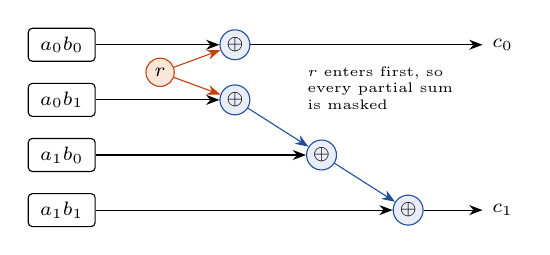
\begin{tikzpicture}[font=\scriptsize,>=Stealth,
 pb/.style={draw,rounded corners=1.5pt,minimum width=0.85cm,minimum height=0.42cm,inner sep=1pt},
 xo/.style={draw=blue,fill=tint,circle,inner sep=0pt,minimum size=0.38cm},
 rr/.style={draw=orange,fill=otint,circle,inner sep=0pt,minimum size=0.36cm}]
\node[pb] (p0) at (0,0) {$a_0b_0$};
\node[pb] (p1) at (0,-0.7) {$a_0b_1$};
\node[pb] (p2) at (0,-1.4) {$a_1b_0$};
\node[pb] (p3) at (0,-2.1) {$a_1b_1$};
\node[rr] (r) at (1.25,-0.35) {$r$};
\node[xo] (x0) at (2.2,0) {$\oplus$};
\node[xo] (x1) at (2.2,-0.7) {$\oplus$};
\node[xo] (x2) at (3.3,-1.4) {$\oplus$};
\node[xo] (x3) at (4.4,-2.1) {$\oplus$};
\node (c0) at (5.6,0) {$c_0$};
\node (c1) at (5.6,-2.1) {$c_1$};
\draw[->] (p0)--(x0); \draw[->] (p1)--(x1); \draw[->] (p2)--(x2); \draw[->] (p3)--(x3);
\draw[->,orange] (r)--(x0); \draw[->,orange] (r)--(x1);
\draw[->,blue] (x1)--(x2); \draw[->,blue] (x2)--(x3);
\draw[->] (x0)--(c0); \draw[->] (x3)--(c1);
\node[align=left,font=\tiny,anchor=west] at (3.0,-0.55) {$r$ enters first, so\\every partial sum\\is masked};
\end{tikzpicture}
\caption{The ISW masked AND: four share products and an XOR chain with one fresh random bit $r$, which enters first so that every partial sum is masked (4 AND + 4 XOR = 8 gates).}\label{fig:isw}
\end{figure}

\subsection{What counts as a leak}
We consider an attacker who can probe one wire (this is called \emph{first order}). A wire \emph{leaks} if what the attacker sees on it depends on the secret, even just statistically (Fig.~\ref{fig:probing}). In the simplest, \emph{glitch-free} model, the attacker sees the wire's final value. Real wires, however, can flicker for a moment while signals arrive \cite{mangard2005glitch}. The \emph{glitch-extended} model \cite{faust2018robust} captures this by letting the probe see everything that feeds into the wire. A \emph{register}, which holds a value steady for one clock tick, blocks this flicker. Our checker decides security exactly, by trying every input and every random bit.

\begin{figure}[!t]
\centering
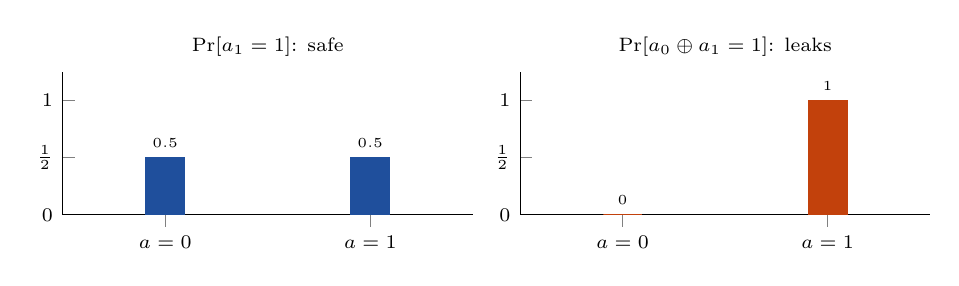
\begin{tikzpicture}
\begin{axis}[name=l,ybar,bar width=14pt,width=0.56\columnwidth,height=3.4cm,ymin=0,ymax=1.25,
 symbolic x coords={a0,a1},xtick=data,xticklabels={$a=0$,$a=1$},ytick={0,0.5,1},yticklabels={0,$\frac12$,1},
 title={$\Pr[a_1=1]$: safe},title style={font=\scriptsize,yshift=-4pt},tick label style={font=\scriptsize},
 nodes near coords,nodes near coords style={font=\tiny},axis lines*=left,enlarge x limits=0.5]
\addplot[fill=blue,draw=blue] coordinates {(a0,0.5)(a1,0.5)};
\end{axis}
\begin{axis}[at={(l.east)},anchor=west,xshift=0.6cm,ybar,bar width=14pt,width=0.56\columnwidth,height=3.4cm,ymin=0,ymax=1.25,
 symbolic x coords={a0,a1},xtick=data,xticklabels={$a=0$,$a=1$},ytick={0,0.5,1},yticklabels={0,$\frac12$,1},
 title={$\Pr[a_0\oplus a_1=1]$: leaks},title style={font=\scriptsize,yshift=-4pt},tick label style={font=\scriptsize},
 nodes near coords,nodes near coords style={font=\tiny},axis lines*=left,enlarge x limits=0.5]
\addplot[fill=orange,draw=orange] coordinates {(a0,0)(a1,1)};
\end{axis}
\end{tikzpicture}
\caption{What a leak looks like. Left: a single share is 1 with probability $\tfrac12$ for both values of the secret (safe). Right: the two shares XORed together reveal the secret exactly (leaks). A wire is safe when $\Pr[w=1\mid a=0]=\Pr[w=1\mid a=1]$.}\label{fig:probing}
\end{figure}

\subsection{PINI}
Checking every input stops being possible for large circuits. PINI \cite{cassiers2020pini} offers a shortcut. A gadget is PINI if a probe inside it can reveal at most one share of each input, and one share alone is just noise. The useful part is that PINI gadgets can be chained: a circuit built only from PINI gadgets is secure at any size. So each gadget is checked once, and the whole circuit never needs to be enumerated.

\subsection{E-graphs and equality saturation}
An e-graph groups expressions that are known to be equal into \emph{e-classes} (Fig.~\ref{fig:egraph}). Equality saturation works in two steps. First, it applies every rewrite rule wherever it can, until nothing new appears; this way the order of the rules no longer matters. Second, it \emph{extracts} a result, normally by picking the cheapest node in each class. Every use of a class then becomes the same wire. One more rule is important later: e-graph equalities must be a \emph{congruence} \cite{suciu2025semantic}, meaning that if $x=y$ then $f(x)=f(y)$ in every context. We use the egglog engine \cite{zhang2023egglog}.

\begin{figure}[!t]
\centering
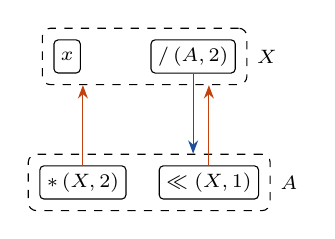
\begin{tikzpicture}[font=\scriptsize,>=Stealth,
 en/.style={draw,rounded corners=1.5pt,inner sep=2.5pt,minimum height=0.42cm},
 ec/.style={draw,dashed,rounded corners=3pt,inner sep=4pt}]
\node[en] (x) at (0,0) {$x$};
\node[en] (div) at (1.6,0) {$/\,(A,2)$};
\node[ec,fit=(x)(div),label={[font=\scriptsize]right:$X$}] (X) {};
\node[en] (mul) at (0.2,-1.6) {$\ast\,(X,2)$};
\node[en] (shl) at (1.8,-1.6) {$\ll(X,1)$};
\node[ec,fit=(mul)(shl),label={[font=\scriptsize]right:$A$}] (A) {};
\draw[->,blue] (div.south) -- (div.south|-A.north);
\draw[->,orange] (mul.north) -- (mul.north|-X.south);
\draw[->,orange] (shl.north) -- (shl.north|-X.south);
\end{tikzpicture}
\caption{An e-graph for $(x\cdot 2)/2$. Dashed boxes are e-classes (sets of equal expressions), solid boxes are e-nodes, and arrows point to operand classes. The cycle records that $(x\cdot 2)/2=x$; nothing is deleted, both forms stay.}\label{fig:egraph}
\end{figure}

\begin{finding}{Key point.}
Saturation finds the options; extraction chooses one. The choice is made on cost alone, with no idea of security. That is where things go wrong.
\end{finding}

% =====================================================================
\section{Finding 1: The Optimiser Breaks Masking}\label{sec:rq1}
% =====================================================================
We start from the ISW gadget and give the optimiser only ordinary, correct rules of Boolean algebra: commutativity, associativity, identities, distributivity and factoring. After saturation the e-graph holds 25 classes and 75 nodes, and the cheapest version has 7 gates instead of 8:
\[
c_0=a_0b_0\oplus r,\qquad c_1=(r\oplus a_0b_1)\oplus a_1(b_0\oplus b_1).
\]
It still computes the right answer on all 32 inputs. But it contains a new wire, $b_0\oplus b_1$, and since $b_1=b\oplus b_0$,
\[
b_0\oplus b_1=b_0\oplus(b\oplus b_0)=b .
\]
That wire \emph{is} the secret $b$ (Fig.~\ref{fig:witness}). One probe reads it directly. We got the same circuit, with the same two leaking wires, on two separate engines (our own e-graph and egglog), and the independent verifier VerifMSI confirms the leak.

\begin{figure}[!t]
\centering
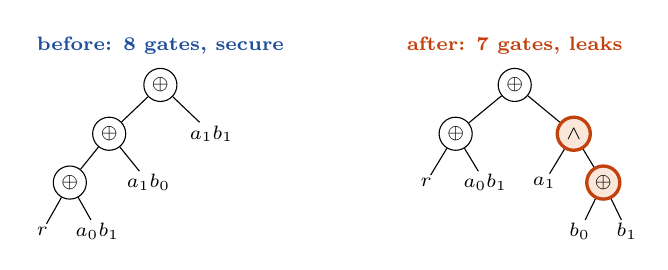
\begin{tikzpicture}[font=\scriptsize,>=Stealth,
  g/.style={draw,circle,inner sep=0.6pt,minimum size=0.42cm},
  lk/.style={g,draw=orange,fill=otint,very thick},
  lf/.style={inner sep=1pt},
  level distance=0.62cm]
\begin{scope}
\node[g] (x3) {$\oplus$}
  child[sibling distance=1.3cm] {node[g] {$\oplus$}
    child[sibling distance=1.0cm] {node[g] {$\oplus$}
      child[sibling distance=0.7cm] {node[lf] {$r$}}
      child[sibling distance=0.7cm] {node[lf] {$a_0b_1$}}}
    child[sibling distance=1.0cm] {node[lf] {$a_1b_0$}}}
  child[sibling distance=1.3cm] {node[lf] {$a_1b_1$}};
\node[above=0.05cm of x3,font=\scriptsize\bfseries,text=blue] {before: 8 gates, secure};
\end{scope}
\begin{scope}[xshift=4.5cm]
\node[g] (y2) {$\oplus$}
  child[sibling distance=1.5cm] {node[g] {$\oplus$}
    child[sibling distance=0.75cm] {node[lf] {$r$}}
    child[sibling distance=0.75cm] {node[lf] {$a_0b_1$}}}
  child[sibling distance=1.5cm] {node[lk] {$\wedge$}
    child[sibling distance=0.75cm] {node[lf] {$a_1$}}
    child[sibling distance=0.75cm] {node[lk] {$\oplus$}
      child[sibling distance=0.6cm] {node[lf] {$b_0$}}
      child[sibling distance=0.6cm] {node[lf] {$b_1$}}}};
\node[above=0.05cm of y2,font=\scriptsize\bfseries,text=orange] {after: 7 gates, leaks};
\end{scope}
\end{tikzpicture}\par\medskip
{\footnotesize$\begin{aligned}
c_1&=\big((r\oplus a_0b_1)\oplus a_1b_0\big)\oplus a_1b_1 &&\text{ISW, 8 gates, secure}\\
c_1&=(r\oplus a_0b_1)\oplus a_1(b_0\oplus b_1) &&\text{factored, 7 gates}\\
b_0\oplus b_1&=b_0\oplus(b\oplus b_0)=\textcolor{orange}{b} &&\text{the new wire is the secret}
\end{aligned}$}\par\medskip
{\footnotesize\begin{tabular}{cccc}
\toprule
$b$ & $b_0$ & $b_1=b\oplus b_0$ & $b_0\oplus b_1$\\\midrule
0&0&0&\textcolor{orange}{\textbf{0}}\\ 0&1&1&\textcolor{orange}{\textbf{0}}\\ 1&0&1&\textcolor{orange}{\textbf{1}}\\ 1&1&0&\textcolor{orange}{\textbf{1}}\\
\bottomrule
\end{tabular}}
\caption{The leak. Factoring $a_1b_0\oplus a_1b_1=a_1(b_0\oplus b_1)$ takes the gadget from 8 gates to 7, but the new wire $b_0\oplus b_1$ equals the secret $b$ in every row of the truth table. The equations give the second output share before and after ($c_0=a_0b_0\oplus r$ in both).}\label{fig:witness}
\end{figure}

\begin{proposition}[Cost-only extraction is unsafe]
There is a secure circuit and a set of correct Boolean rewrite rules for which the cheapest extracted circuit is insecure.
\end{proposition}
The example above is the proof. No rule is wrong; the leaking circuit wins only because it is cheaper.

\begin{finding}{Why the cheaper circuit leaks.}
This is not a coincidence. A two-share gadget turns $a\wedge b$ into four share products. Reordering and regrouping them never saves a gate; only factoring out a common term does. Two products share a term only if they share a share index, and factoring them then gives $a_i(b_0\oplus b_1)=a_i\wedge b$, or the same with $a$ and $b$ swapped. So with two shares, \textbf{every gate-saving factoring puts a secret back together}.
\end{finding}

\subsection{Is this only a two-share effect?}\label{sec:shares}
With $d\ge 3$ shares the argument above weakens, because $b_0\oplus b_1$ is a uniform bit rather than the secret. We therefore repeated the search for the $d$-share ISW gadget, enumerating every way to reorder the XOR terms and to factor products that share an index, and checking each wire exactly (Table~\ref{tab:shares}). We built the cheapest secure circuit and a cost-only circuit as netlists for each $d$ and checked every wire against VerifMSI: no disagreement on any of the 159 wires. The cost-only optimum still leaks for $d=3$ and $d=4$, because the last output share contains all $d$ products with one index, and factoring them gives $a_{d-1}\wedge b$. The difference is that \emph{secure} savings now exist, such as $a_2(b_0\oplus b_1)$ for $d=3$. So ``every gate-saving factoring recombines a secret'' is a two-share statement; the weaker statement ``the cheapest circuit found by cost alone leaks'' holds up to $d=4$ in this model. This is a first-order, glitch-free measurement of the gadget only; it does not cover refreshes, DOM or HPC structure, or higher-order probing.

\begin{table}[t]
\caption{Cost-Only Versus Secure Optimum for the $d$-Share ISW AND (Gates, Shared Gates Counted Once; First Order, Glitch-Free)}\label{tab:shares}
\centering\footnotesize
\begin{tabular}{@{}rrrr@{}}
\toprule
Shares $d$ & Plain ISW & Cost-only & Cheapest secure\\\midrule
2 & 8 & 7, \bad & 8\\
3 & 21 & 16, \bad & 17\\
4 & 40 & 27, \bad & 28\\
\bottomrule
\end{tabular}
\end{table}

% =====================================================================
\section{Finding 2: Checking Security at Extraction Fixes It}\label{sec:rq2}
% =====================================================================
In the glitch-free model, whether a wire leaks depends only on the function it computes. That means we can label each e-class as safe or unsafe once, and reuse the label. The fix has three steps (Fig.~\ref{fig:repair}):
\begin{enumerate}
\item label every e-class safe or unsafe;
\item pick the cheapest circuit, but never use an unsafe class as an internal wire;
\item check the result again with an independent tool.
\end{enumerate}
The rules and the e-graph stay exactly the same; only the choice changes. The result is the secure 8-gate ISW gadget again (Table~\ref{tab:wire}). \textbf{Security costs one gate.}

\begin{table}[t]
\caption{Wire-Level Results on ISW (Cost: Gates)}\label{tab:wire}
\centering\footnotesize
\begin{tabular}{@{}lccl@{}}
\toprule
Rule set & Classes & Gates & Security\\\midrule
Core (commute, associate, identities) & 23 & 8 & \ok\\
Full (+ distributivity, factoring), cost only & 25 & 7 & \bad\\
Full, constrained extraction & 25 & 8 & \ok\\
\bottomrule
\end{tabular}
\end{table}
\begin{figure}[!t]
\centering
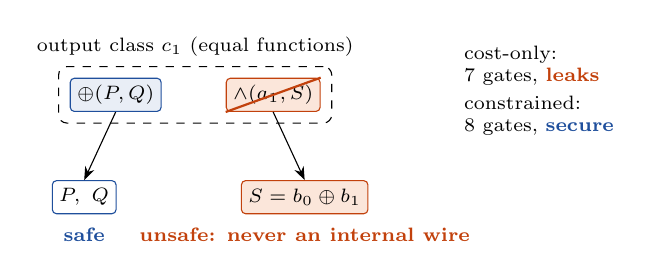
\begin{tikzpicture}[font=\scriptsize,>=Stealth,
 en/.style={draw,rounded corners=1.5pt,inner sep=2.5pt,minimum height=0.42cm},
 ec/.style={draw,dashed,rounded corners=3pt,inner sep=4pt}]
\node[en,draw=blue,fill=tint] (pq) at (0,0) {$\oplus(P,Q)$};
\node[en,draw=orange,fill=otint] (as) at (2.0,0) {$\wedge(a_1,S)$};
\node[ec,fit=(pq)(as),label={[font=\scriptsize]above:output class $c_1$ (equal functions)}] (C) {};
\draw[orange,thick] (as.south west)--(as.north east);
\node[en,draw=blue] (P) at (-0.4,-1.3) {$P,\ Q$};
\node[en,draw=orange,fill=otint] (S) at (2.4,-1.3) {$S=b_0\oplus b_1$};
\draw[->] (pq.south) -- (P.north);
\draw[->] (as.south) -- (S.north);
\node[font=\scriptsize\bfseries,text=blue,below=0.05cm of P] {safe};
\node[font=\scriptsize\bfseries,text=orange,below=0.05cm of S] {unsafe: never an internal wire};
\node[align=left,anchor=west,font=\scriptsize] at (4.3,0.05) {cost-only:\\ 7 gates, \textcolor{orange}{\textbf{leaks}}\\[2pt] constrained:\\ 8 gates, \textcolor{blue}{\textbf{secure}}};
\end{tikzpicture}
\caption{Security-constrained extraction. Same rules and same e-graph; every class is labelled safe or unsafe, and the unsafe class $S=b_0\oplus b_1$ is never used as an internal wire. Ignoring security gives 7 gates and leaks; enforcing it gives 8 gates and is secure.}\label{fig:repair}
\end{figure}

\emph{Why not simply ban the factoring rule?} Three reasons. Factoring is useful elsewhere (later it takes a circuit from 20 to 11 and stays secure). Other moves leak too, such as moving $r$ to the end in ISW or dropping a needed refresh. And a leak depends on which wires end up in the circuit, not on which rule produced them. So we let every rule fire and check the result.

\emph{Is there a cheaper secure circuit somewhere?} We tried a larger example: two ISW gadgets in a row, computing $(a\wedge b)\wedge d$, which takes 16 gates by hand and is secure. We combined the 40 cheapest options for each of its two outputs, across 6 variants of the e-graph, giving 240 circuits. Not one is secure, and the 28 that are cheaper than the hand design all leak (Fig.~\ref{fig:chain}). This is a sample, not a proof, but the message is clear: ordinary algebra alone gives no free savings here. The reason has to do with how the circuit is represented, which is the next finding.

\begin{figure}[!t]
\centering
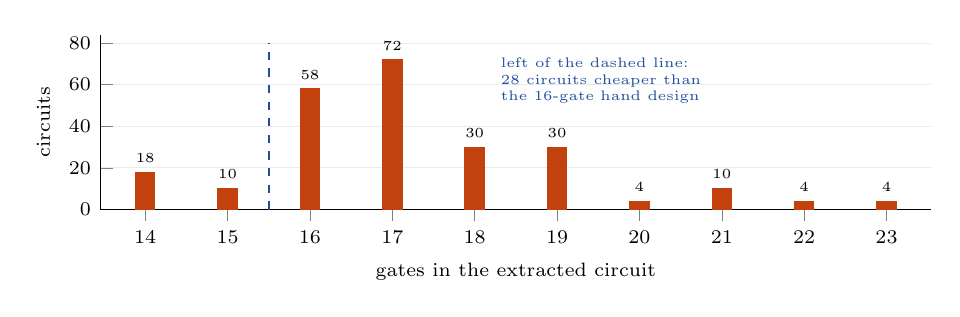
\begin{tikzpicture}
\begin{axis}[ybar,bar width=7pt,width=\columnwidth,height=3.8cm,
 ymin=0,ymax=84,xlabel={gates in the extracted circuit},ylabel={circuits},
 xtick={14,...,23},xticklabel style={font=\scriptsize},yticklabel style={font=\scriptsize},
 label style={font=\scriptsize},nodes near coords,nodes near coords style={font=\tiny},
 axis lines*=left,ymajorgrids,grid style={black!8},enlarge x limits=0.06]
\addplot[fill=orange,draw=orange] coordinates {(14,18)(15,10)(16,58)(17,72)(18,30)(19,30)(20,4)(21,10)(22,4)(23,4)};
\draw[blue,thick,dashed] (axis cs:15.5,0) -- (axis cs:15.5,80);
\node[font=\tiny,text=blue,anchor=west,align=left] at (axis cs:18.2,62) {left of the dashed line:\\28 circuits cheaper than\\the 16-gate hand design};
\end{axis}
\end{tikzpicture}
\caption{Chain scale. Gate counts of the 240 sampled extractions of a two-gadget ISW chain: none is secure, and the 28 that beat the 16-gate hand design all leak. VerifMSI agrees on all 6,054 wires.}\label{fig:chain}
\end{figure}

% =====================================================================
\section{Finding 3: Designers' Tricks Do Not Fit a Standard E-Graph}\label{sec:rq3}
% =====================================================================
Masking designers save cost with a different set of moves: refreshes, gadget swaps and registers (Fig.~\ref{fig:resharing}). All of them keep the \emph{secret} the same and change the \emph{shares}. We call this \emph{re-sharing}.

\begin{figure}[!t]
\centering
{\footnotesize\begin{tabularx}{\columnwidth}{@{}l>{\raggedright\arraybackslash}X@{}}
\toprule
Move & What it does\\\midrule
Refresh & $(x_0,x_1)\mapsto(x_0\oplus r,\,x_1\oplus r)$: same secret, fresh shares\\
Gadget swap & $\mathrm{ISW}(a,b)\leftrightarrow\mathrm{DOM}(a,b)$: same product, different wires\\
Register & holds a value steady; to a probe under glitches it acts like a refresh\\
Random-bit reuse & one random bit shared between gadgets (not modelled here)\\
\bottomrule
\end{tabularx}}
\caption{Re-sharing: the moves masking designers use. All four keep the secret and change the shares.}\label{fig:resharing}
\end{figure}

\begin{finding}{Finding 3.}
Let $y$ be a refresh of $x$, so $y_0=x_0\oplus r$ and $y_1=x_1\oplus r$. Both hold the same secret. Now look only at share 0: whenever $r=1$, $x_0$ and $y_0$ differ. So $x$ and $y$ are equal as secrets but not as wires. That breaks the congruence rule, and \textbf{a correct wire-level e-graph is never allowed to treat them as equal} (Fig.~\ref{fig:congruence}).
\end{finding}

\begin{figure}[!t]
\centering
$x=y\ \Rightarrow\ f(x)=f(y)$\par\smallskip
{\footnotesize\setlength{\tabcolsep}{5pt}\begin{tabular}{ccccccc}
\toprule
$x$ & $y$ & $r$ & $x_0$ & $y_0=x_0\oplus r$ & $x_1$ & $y_1=x_1\oplus r$\\\midrule
1&1&0&1&1&0&0\\
1&1&0&0&0&1&1\\
0&0&1&0&\textcolor{orange}{\textbf{1}}&0&1\\
1&1&1&0&\textcolor{orange}{\textbf{1}}&1&0\\
\bottomrule
\end{tabular}}
\caption{Why re-sharing is not a congruence. $x$ and $y=\rf(x)$ always hold the same secret (columns $x$ and $y$), but share 0 differs in rows 3 and 4, so the context ``read share 0 gives $f(x)=0$ and $f(y)=1$.''}\label{fig:congruence}
\end{figure}

In other words, a wire-level optimiser cannot even \emph{see} the designers' moves. We found no earlier statement of this point for e-graphs.

\subsection{A second e-graph, over secret values}
Our answer is to move the e-graph up a level, so that each class stands for a secret value rather than a particular set of wires (Fig.~\ref{fig:value}). A term is built from inputs, XOR, NOT, refresh, registers and gadgets:
\[
x ::= \mathsf{in}(s)\mid \mathsf{xor}(x,x)\mid\mathsf{not}(x)\mid\rf(x)\mid\reg(x)\mid g(x,x),
\]
where $g$ is one of $\isw$, $\dom$ or $\hpc$. Its value is what you would expect: $\val{g(x,y)}=\val x\wedge\val y$, and refresh and registers do not change the value. Three groups of rules act on it: \textbf{R1} is ordinary Boolean algebra on values (including factoring), \textbf{R2} says the three gadgets are interchangeable, and \textbf{R3} says a refresh can be removed. To measure cost, we turn a term back into a two-share circuit (\emph{lowering}), with a fresh random bit for every gadget and refresh, and count gates plus random bits.

\begin{figure}[!t]
\centering
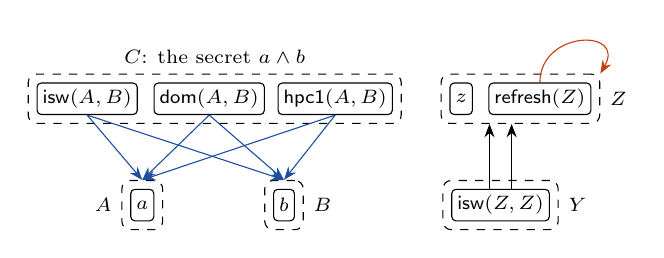
\begin{tikzpicture}[font=\scriptsize,>=Stealth,
 en/.style={draw,rounded corners=1.5pt,inner sep=2pt,minimum height=0.4cm},
 ec/.style={draw,dashed,rounded corners=3pt,inner sep=3pt}]
\node[en] (i) at (0,0) {$\isw(A,B)$};
\node[en] (d) at (1.55,0) {$\dom(A,B)$};
\node[en] (h) at (3.15,0) {$\hpc(A,B)$};
\node[ec,fit=(i)(h),label={[font=\scriptsize]above:$C$: the secret $a\wedge b$}] (C) {};
\node[en] (a) at (0.7,-1.35) {$a$}; \node[ec,fit=(a),label={[font=\scriptsize]left:$A$}] (A) {};
\node[en] (b) at (2.5,-1.35) {$b$}; \node[ec,fit=(b),label={[font=\scriptsize]right:$B$}] (Bc) {};
\foreach \n in {i,d,h}{\draw[->,blue] (\n.south)--(A.north); \draw[->,blue] (\n.south)--(Bc.north);}
\node[en] (z) at (4.75,0) {$z$};
\node[en] (rz) at (5.75,0) {$\rf(Z)$};
\node[ec,fit=(z)(rz),label={[font=\scriptsize]right:$Z$}] (Z) {};
\draw[->,orange] (rz.north) to[out=90,in=60,looseness=2.2] (Z.north east);
\node[en] (sq) at (5.25,-1.35) {$\isw(Z,Z)$};
\node[ec,fit=(sq),label={[font=\scriptsize]right:$Y$}] (Y) {};
\draw[->] ([xshift=-4pt]sq.north)--([xshift=-4pt]sq.north|-Z.south);
\draw[->] ([xshift=4pt]sq.north)--([xshift=4pt]sq.north|-Z.south);
\end{tikzpicture}
\caption{The value-level e-graph. A class stands for a secret value: three gadgets build the same value $a\wedge b$ (R2), and a refresh joins its own class as a self-loop (R3).}\label{fig:value}
\end{figure}

\begin{proposition}[The value-level rules are safe to use]
If $\val x=\val{x'}$ and $\val y=\val{y'}$, then $\val{\mathsf{op}(x,y)}=\val{\mathsf{op}(x',y')}$, so R1--R3 are valid e-graph rules. Lowering is also correct: the output shares of a lowered term always XOR to its value.
\end{proposition}
\emph{Proof.} The value of a term is defined piece by piece from the values of its parts, and lowering is correct by induction (a refresh is correct because $r$ cancels out, and each gadget by its own correctness).\hfill$\square$

Notice that security is no longer part of the equality at all. It has to be enforced when the circuit is chosen, and that is where the next surprise appears.

% =====================================================================
\section{Finding 4: One Label Per Class Is No Longer Enough}\label{sec:extract}
% =====================================================================
\begin{proposition}[Safety is not a property of the e-class]\label{prop:vplc}
With refresh removal (R3), $\isw(z,z)$ and $\isw(z,\rf(z))$ end up in the same e-class, yet the first leaks and the second is secure. Picking one node per class always returns $\isw(z,z)$, while picking whole terms can return the secure one.
\end{proposition}
Here is the intuition. In $\isw(z,z)$, both inputs are the same pair of shares, so one product wire is 1 half the time when $z=0$ and never when $z=1$; it leaks $z$. With a refresh on one input, every product wire is 1 a quarter of the time, whatever $z$ is (Fig.~\ref{fig:class}). Because R3 makes the refresh a loop back into $z$'s own class, the usual one-node-per-class extraction cannot use it, so both inputs become the same wire (full proof in Appendix~\ref{app:proofs}). This is a statement about this rule set: with all three rule groups, 16 of the 338 possible one-node-per-class choices are secure, and at the wire level a single label per class still works.

\begin{figure*}[!t]
\centering
{\footnotesize
\begin{tabular}[t]{cccc}
\multicolumn{4}{c}{\textcolor{orange}{\textbf{$\isw(z,z)$: leaks}}}\\\toprule
$z$ & $z_0$ & $z_1$ & $z_0z_1$\\\midrule
0&0&0&0\\ 0&1&1&\textcolor{orange}{\textbf{1}}\\ 1&0&1&0\\ 1&1&0&0\\\bottomrule
\end{tabular}\hspace{2.2em}
\begin{tabular}[t]{cccccc}
\multicolumn{6}{c}{\textcolor{blue}{\textbf{$\isw(z,\rf(z))$: secure}}}\\\toprule
$z$ & $z_0$ & $r$ & $z_1$ & $z_1'=z_1\oplus r$ & $z_0z_1'$\\\midrule
0&0&0&0&0&0\\ 0&0&1&0&1&0\\ 0&1&0&1&1&\textcolor{blue}{\textbf{1}}\\ 0&1&1&1&0&0\\
1&0&0&1&1&0\\ 1&0&1&1&0&0\\ 1&1&0&0&0&0\\ 1&1&1&0&1&\textcolor{blue}{\textbf{1}}\\\bottomrule
\end{tabular}}
\caption{Why one safe-or-unsafe label per class fails. Left, $\isw(z,z)$: both operands are one sharing, and the product wire $z_0z_1$ is 1 in one of two cases when $z=0$ and never when $z=1$, so it leaks $z$. Right, $\isw(z,\rf(z))$: the product is 1 in one of four cases for either value of $z$, so it is safe. Refresh removal puts both terms in one e-class.}\label{fig:class}
\end{figure*}

\subsection{Safe method 1: check each candidate, cut leaks early}
Instead of choosing one node per class, we choose whole \emph{terms}, so the same class can be built differently in different places. Each class keeps its $k=8$ cheapest terms (the results were identical for $k=2$, 8 and 32 on the value-layer fixtures, but not on the $2{\times}2$ multiplier, where the secure optimum is 69 for $k$ from 2 to 8 and 75 for $k=16$ and 32, so extraction is a search: the costs we report are the best found, not proven optima). Each candidate is lowered to wires, and every wire is checked exactly.

\begin{proposition}[Leak cut]\label{prop:cut}
In both models, if a piece of a circuit has a leaking wire, then every larger circuit containing that piece also leaks.
\end{proposition}
So a leaking piece can be thrown away as soon as it is found, and every result is secure by construction. On the squaring example, $\isw(z,z)$ (cost 11) is cut and $\isw(z,\rf(z))$ (cost 14) is kept. The price is speed: 0.3\,s on a chain of depth 3, 5.4\,s at depth 4 and 133\,s at depth 5.

\subsection{Safe method 2: PINI brings back one label per class}
We call a class \emph{composable} if it contains a PINI gadget whose inputs are also composable. We checked each operator exhaustively and with VerifMSI: XOR, NOT, refresh and HPC1 are PINI, while ISW and DOM are not. Inside composable classes a single safe label works again, and the usual one-node-per-class extraction is safe, \textbf{without checking any inputs at all}. This is what lets the method scale.

% =====================================================================
\section{Results}\label{sec:results}
% =====================================================================
\subsection{Savings appear only where there is waste}
Fig.~\ref{fig:slack} shows the cheapest secure circuit found from several starting points. Every saving comes from one of two kinds of waste: a refresh that was not needed, or two products that can be factored. Circuits that are already tight do not move. VerifMSI confirms every secure result (27 circuits, 914 wires). The security check still matters at this level: if refresh removal is allowed, a cost-only optimiser returns $\isw(z,z)$ (cost 11, leaks) instead of $\isw(z,\rf(z))$ (cost 14, secure).

\begin{figure}[!t]
\centering
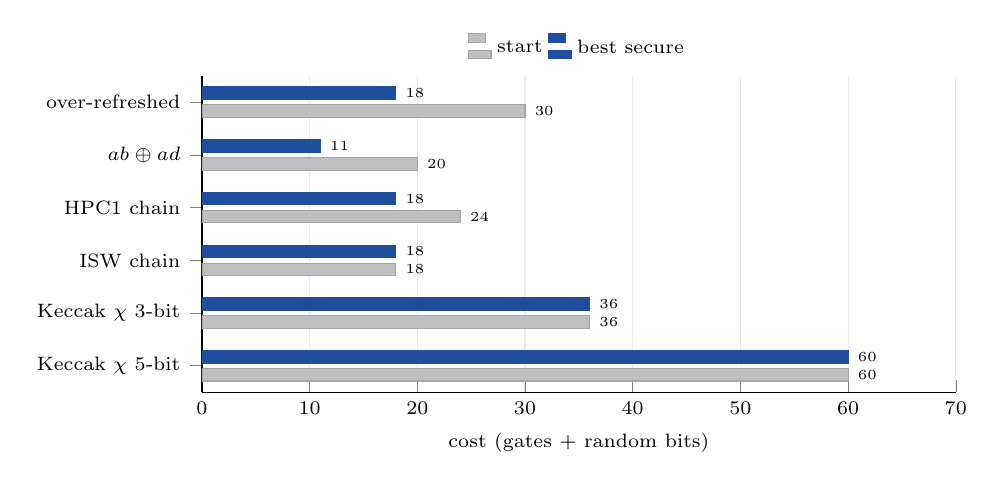
\begin{tikzpicture}
\begin{axis}[xbar,bar width=4.5pt,width=0.92\columnwidth,height=5.6cm,
 xmin=0,xmax=70,xlabel={cost (gates + random bits)},
 symbolic y coords={chi5,chi3,chain,hpc,factor,overref},ytick=data,
 yticklabels={Keccak $\chi$ 5-bit,Keccak $\chi$ 3-bit,ISW chain,HPC1 chain,$ab\oplus ad$,over-refreshed},
 yticklabel style={font=\scriptsize},xticklabel style={font=\scriptsize},label style={font=\scriptsize},
 nodes near coords,nodes near coords style={font=\tiny},
 legend style={font=\scriptsize,at={(0.5,1.02)},anchor=south,draw=none,legend columns=2},
 axis lines*=left,xmajorgrids,grid style={black!8},enlarge y limits=0.1]
\addplot[fill=black!25,draw=black!35] coordinates {(60,chi5)(36,chi3)(18,chain)(24,hpc)(20,factor)(30,overref)};
\addplot[fill=blue,draw=blue] coordinates {(60,chi5)(36,chi3)(18,chain)(18,hpc)(11,factor)(18,overref)};
\legend{start,best secure}
\end{axis}
\end{tikzpicture}
\caption{Value-layer results (cost = gates + random bits). Refresh removal, factoring and gadget swaps save cost where the start circuit had slack: over-refreshed chain 30 to 18 (R3), two ANDs sharing a factor 20 to 11 (R1), HPC1 chain 24 to 18 (R2, glitch-free only). The hand-written chain and Keccak $\chi$ are tight and do not improve.}\label{fig:slack}
\end{figure}

Table~\ref{tab:ablation} switches the three rule groups on and off. Each saving has one source: refresh removal (R3) gives the over-refreshed chain, Boolean algebra with factoring (R1) gives the shared-factor program, and gadget swaps (R2) give the HPC1 chain. No other combination saves anything, and the only configurations whose cost-only optimum leaks are those that contain R3.

\begin{table}[t]
\caption{Rule Ablation: Cheapest Secure Cost (Gates + Random Bits); ``11 leaks'' Is the Cost-Only Optimum When It Differs}\label{tab:ablation}
\centering\scriptsize
\setlength{\tabcolsep}{2.6pt}
\begin{tabular}{@{}lrcccccccc@{}}
\toprule
Circuit & Start & none & R1 & R2 & R3 & R1+R2 & R1+R3 & R2+R3 & all\\\midrule
ISW chain & 18 & 18 & 18 & 18 & 18 & 18 & 18 & 18 & 18\\
over-refreshed & 30 & 30 & 30 & 30 & \textbf{18} & 30 & \textbf{18} & \textbf{18} & \textbf{18}\\
$z\wedge z$ & 14 & 14 & 14 & 14 & \makecell{14\\\textcolor{orange}{11 leaks}} & 14 & \makecell{14\\\textcolor{orange}{11 leaks}} & \makecell{14\\\textcolor{orange}{11 leaks}} & \makecell{14\\\textcolor{orange}{11 leaks}}\\
$ab\oplus ad$ & 20 & 20 & \textbf{11} & 20 & 20 & \textbf{11} & \textbf{11} & 20 & \textbf{11}\\
HPC1 chain & 24 & 24 & 24 & \textbf{18} & 24 & \textbf{18} & 24 & \textbf{18} & \textbf{18}\\
Keccak $\chi$, 5-bit & 60 & 60 & 60 & 60 & 60 & 60 & 60 & 60 & 60\\
\bottomrule
\end{tabular}
\end{table}

\subsection{Finding 5: glitches and large circuits}\label{sec:rq4}
\emph{Glitches.} A glitch is a brief wrong value on a wire while signals are still arriving (Fig.~\ref{fig:glitch}). A register blocks it, so to an attacker a register works like a refresh. To a cost-only optimiser, however, a register looks like a wire that does nothing, so it deletes it (Table~\ref{tab:glitch}). Our check puts the registers back, and on the unregistered ISW gadget it adds two registers exactly where they are needed. Of egglog's own 784 cheapest candidates for a DOM chain, none is glitch-secure. Our glitch checker agrees with VerifMSI on all 167 probes.

\begin{figure}[!t]
\centering
$w=(a_0\oplus r)\oplus a_1$, with $a=1$, $a_0=0$, $a_1=1$, $r=1$\par\smallskip
{\footnotesize\begin{tabularx}{\columnwidth}{@{}l>{\raggedright\arraybackslash}Xccl@{}}
\toprule
Time & Event & $u=a_0\oplus r$ & $w=u\oplus a_1$ & Wire holds\\\midrule
$t_0$ & nothing has arrived & 0 & 0 & nothing useful\\
$t_1$ & $a_0,a_1$ arrive; $r$ still 0 & 0 & \textcolor{orange}{\textbf{1}} & \textcolor{orange}{\textbf{the secret $a$}}\\
$t_2$ & $r=1$ arrives & 1 & 0 & $a\oplus r$, random\\
\bottomrule
\end{tabularx}}
\caption{A glitch. While signals arrive, the wire $w=(a_0\oplus r)\oplus a_1$ briefly holds the secret $a$ before $r$ arrives; its final value passes a basic check. A probe that sees the wire's history sees $a$, and a register stops this.}\label{fig:glitch}
\end{figure}
\begin{table}[t]
\caption{Registers Under Glitches (Cost: Gates + Registers)}\label{tab:glitch}
\centering\footnotesize
\begin{tabular}{@{}lrrr@{}}
\toprule
Circuit & Start & Registers ignored & Constrained\\\midrule
Registered DOM AND & 10 & 5, \bad & 10, \ok\\
DOM chain (registered) & 20 & 10, \bad & 20, \ok\\
ISW AND, no registers & 8 & 7, \bad & 10, \ok\\
DOM AND, no registers & 8 & 5, \bad & 10, \ok\\
\bottomrule
\end{tabular}
\end{table}

\emph{Large circuits.} Checking every input stops at around $2^{26}$ combinations. PINI-based extraction does not need to enumerate anything (Table~\ref{tab:pini}), and none of 234 randomly built PINI circuits leaks. The price is size: an HPC1 gadget costs 12 where ISW costs 9, so PINI results are 25--33\% larger. This result holds in the glitch-free model.

\begin{table}[t]
\caption{Exact Checking Versus PINI Composition}\label{tab:pini}
\centering\footnotesize
\setlength{\tabcolsep}{4pt}
\begin{tabular}{@{}lrllrr@{}}
\toprule
Circuit & Inputs & Exact & PINI & Time & VerifMSI\\\midrule
Keccak $\chi$, 6-bit & $2^{24}$ & secure & secure & 0.01\,s & 103/103\\
Keccak $\chi$, 8-bit & $2^{32}$ & too large & secure & 0.01\,s & 137/137\\
Keccak $\chi$, 32-bit & $2^{128}$ & too large & secure & 0.05\,s & 545/545\\
ISW chain, depth 15 & $2^{62}$ & too large & secure & 0.01\,s & 212/212\\
\bottomrule
\end{tabular}
\end{table}

% =====================================================================
\section{System Architecture}\label{sec:arch}
% =====================================================================
Fig.~\ref{fig:arch} shows how the tool is organised, in four layers. The \emph{front end} reads a program and masks it. The \emph{optimiser} holds the two e-graphs and the two ways of choosing a circuit. The \emph{oracles} are the security checkers that the optimiser consults. The \emph{back end} checks the result and writes it out, and a test harness reruns everything. Table~\ref{tab:components} describes each part in one line.

\begin{figure*}[!t]
\centering
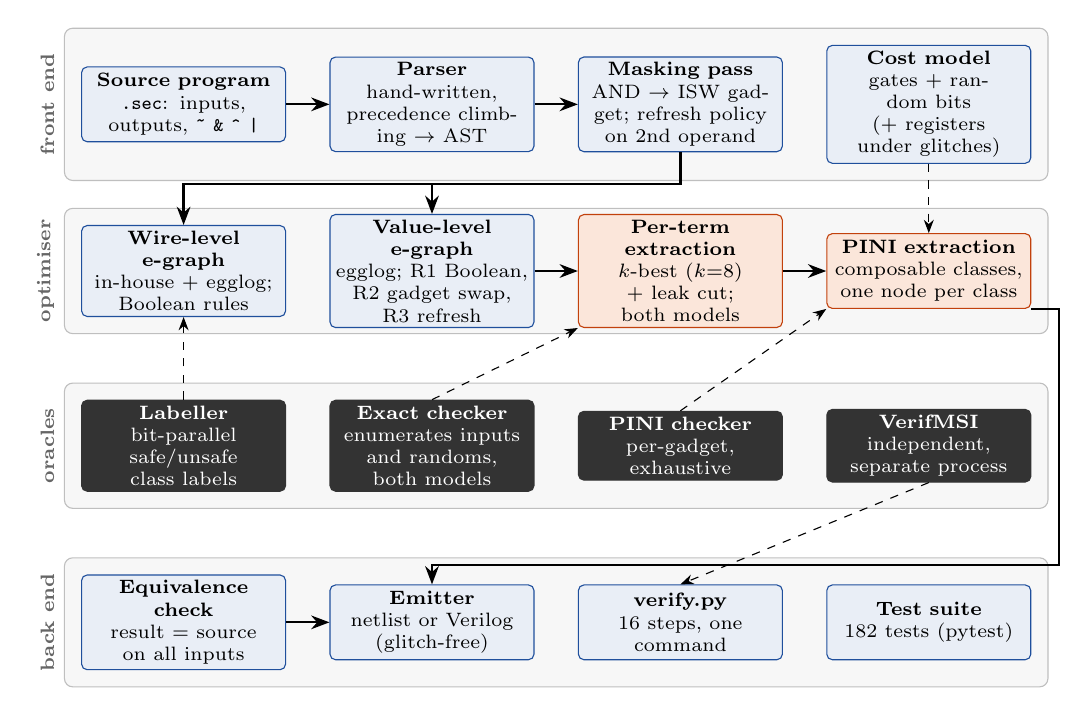
\begin{tikzpicture}[font=\scriptsize,>=Stealth,
  lay/.style={draw=black!25,fill=black!3,rounded corners=3pt,inner sep=5pt},
  box/.style={draw=blue,fill=tint,rounded corners=2pt,minimum height=0.95cm,text width=2.45cm,align=center,inner sep=2pt},
  hot/.style={box,draw=orange,fill=otint},
  ora/.style={draw=black!80,fill=black!80,text=white,rounded corners=2pt,minimum height=0.85cm,text width=2.45cm,align=center,inner sep=2pt},
  lab/.style={font=\scriptsize\bfseries,text=black!60,anchor=west}]
% layer 1
\node[box] (src) {\textbf{Source program}\\ \texttt{.sec}: inputs, outputs, \texttt{\textasciitilde\ \& \textasciicircum\ |}};
\node[box,right=0.55cm of src] (par) {\textbf{Parser}\\ hand-written, precedence climbing $\to$ AST};
\node[box,right=0.55cm of par] (msk) {\textbf{Masking pass}\\ AND $\to$ ISW gadget; refresh policy on 2nd operand};
\node[box,right=0.55cm of msk] (cost) {\textbf{Cost model}\\ gates + random bits\\ (+ registers under glitches)};
% layer 2
\node[box,below=1.05cm of src] (wire) {\textbf{Wire-level e-graph}\\ in-house + egglog;\\ Boolean rules};
\node[box,right=0.55cm of wire] (val) {\textbf{Value-level e-graph}\\ egglog; R1 Boolean, R2 gadget swap, R3 refresh};
\node[hot,right=0.55cm of val] (ext1) {\textbf{Per-term extraction}\\ $k$-best ($k{=}8$) + leak cut; both models};
\node[hot,right=0.55cm of ext1] (ext2) {\textbf{PINI extraction}\\ composable classes, one node per class};
% layer 3
\node[ora,below=1.05cm of wire] (lab) {\textbf{Labeller}\\ bit-parallel safe/unsafe class labels};
\node[ora,right=0.55cm of lab] (ex) {\textbf{Exact checker}\\ enumerates inputs and randoms, both models};
\node[ora,right=0.55cm of ex] (pini) {\textbf{PINI checker}\\ per-gadget, exhaustive};
\node[ora,right=0.55cm of pini] (vm) {\textbf{VerifMSI}\\ independent, separate process};
% layer 4
\node[box,below=1.05cm of lab] (eq) {\textbf{Equivalence check}\\ result = source on all inputs};
\node[box,right=0.55cm of eq] (emit) {\textbf{Emitter}\\ netlist or Verilog (glitch-free)};
\node[box,right=0.55cm of emit] (ver) {\textbf{verify.py}\\ 16 steps, one command};
\node[box,right=0.55cm of ver] (tst) {\textbf{Test suite}\\ 182 tests (pytest)};
% layer frames
\begin{scope}[on background layer]
\node[lay,fit=(src)(cost),inner xsep=6pt,inner ysep=6pt] (L1) {};
\node[lay,fit=(wire)(ext2),inner xsep=6pt,inner ysep=6pt] (L2) {};
\node[lay,fit=(lab)(vm),inner xsep=6pt,inner ysep=6pt] (L3) {};
\node[lay,fit=(eq)(tst),inner xsep=6pt,inner ysep=6pt] (L4) {};
\end{scope}
\node[lab,rotate=90,anchor=south] at (L1.west) {front end};
\node[lab,rotate=90,anchor=south] at (L2.west) {optimiser};
\node[lab,rotate=90,anchor=south] at (L3.west) {oracles};
\node[lab,rotate=90,anchor=south] at (L4.west) {back end};
% arrows
\draw[->,thick] (src)--(par); \draw[->,thick] (par)--(msk);
\draw[->,thick] (msk.south) -- ++(0,-0.4) -| (val.north);
\draw[->,thick] (msk.south) -- ++(0,-0.4) -| (wire.north);
\draw[->,thick] (val)--(ext1); \draw[->,thick] (ext1)--(ext2);
\draw[->,dashed] (cost.south)--(ext2.north);
\draw[->,dashed] (lab.north)--(wire.south);
\draw[->,dashed] (ex.north)--(ext1.south west);
\draw[->,dashed] (pini.north)--(ext2.south west);
\draw[->,thick] (ext2.south east) -- ++(0.35,0) |- ([yshift=0.25cm]emit.north) -- (emit.north);
\draw[->,thick] (eq)--(emit);
\draw[->,dashed] (vm.south)--(ver.north);
\end{tikzpicture}
\caption{Architecture of the tool. Solid arrows are the compilation flow; dashed arrows show which oracle each stage consults. Extraction (orange) is the only optimisation stage that depends on security; VerifMSI is never linked into our code and is used only to cross-check.}
\label{fig:arch}
\end{figure*}
\begin{table}[t]
\caption{Components of the Tool}\label{tab:components}
\centering\footnotesize
\begin{tabularx}{\columnwidth}{@{}>{\bfseries\raggedright\arraybackslash}p{2.5cm}>{\raggedright\arraybackslash}X@{}}
\toprule
Component & Role\\\midrule
Parser & Reads the source language; one syntax tree per output.\\
Masking pass & Two shares per value; ISW per AND; refresh policy keeps operand sharings independent.\\
Wire-level e-graph & Boolean rewriting of masked wires (RQ1, RQ2); our own engine and an egglog port.\\
Value-level e-graph & One class per secret value; R1--R3 as rules (RQ3).\\
Per-term extraction & $k$ cheapest terms per class, lowered and checked; leaking terms cut for good.\\
PINI extraction & Class-level extraction on composable classes; no enumeration (RQ4).\\
Labeller & Bit-parallel safe/unsafe labels; 0.4\,s for a depth-5 chain against an estimated 61\,min for the reference labeller.\\
Exact checker & Ground truth for first-order security, glitch-free and glitch-extended.\\
VerifMSI & External oracle; any disagreement stops the work until fixed.\\
Emitter & Netlist or Verilog with \texttt{a\_s0}, \texttt{a\_s1}, \ldots{} ports.\\
\bottomrule
\end{tabularx}
\end{table}

% =====================================================================
\section{The seqc Compiler}\label{sec:compiler}
% =====================================================================
Fig.~\ref{fig:pipeline} follows a program through the compiler. The front end reads a small language with \code{input}, \code{out} and the operators \code{\textasciitilde}, \code{\&}, \code{\textasciicircum} and \code{|}. The masking pass turns each AND into an ISW gadget and refreshes its second input. egglog then saturates the e-graph with rules R1--R3. Extraction runs twice, once ignoring security and once enforcing it, so the cost of security is always visible. The result is checked (same output as the source on every input, no leaking wire, VerifMSI agrees) and written out as a netlist or Verilog. The Verilog is marked as secure in the glitch-free model only.

\begin{figure*}[t]
\centering
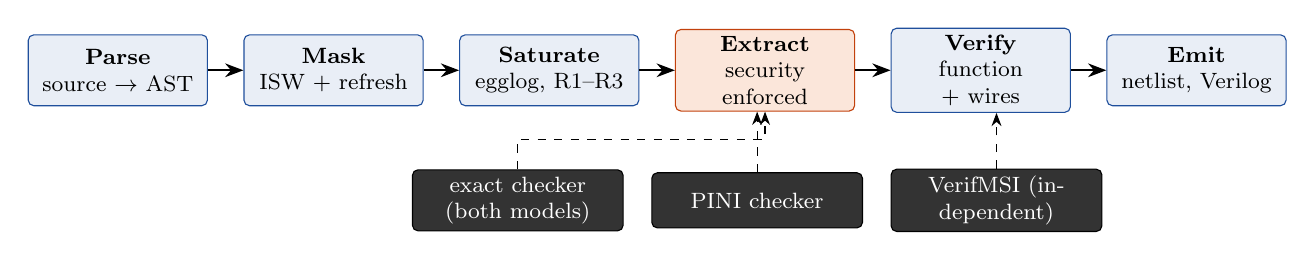
\begin{tikzpicture}[font=\footnotesize,>=Stealth,
  box/.style={draw=blue,fill=tint,rounded corners=2pt,minimum height=0.9cm,text width=2.1cm,align=center,inner sep=2.5pt},
  hi/.style={box,draw=orange,fill=otint},
  chk/.style={draw,fill=black!80,text=white,rounded corners=2pt,minimum height=0.7cm,text width=2.5cm,align=center,inner sep=2.5pt}]
\node[box] (p) {\textbf{Parse}\\ source $\to$ AST};
\node[box,right=0.45cm of p] (m) {\textbf{Mask}\\ ISW + refresh};
\node[box,right=0.45cm of m] (e) {\textbf{Saturate}\\ egglog, R1--R3};
\node[hi,right=0.45cm of e] (x) {\textbf{Extract}\\ security enforced};
\node[box,right=0.45cm of x] (v) {\textbf{Verify}\\ function + wires};
\node[box,right=0.45cm of v] (o) {\textbf{Emit}\\ netlist, Verilog};
\foreach \a/\b in {p/m,m/e,e/x,x/v,v/o} \draw[->,thick] (\a)--(\b);
\node[chk,below=0.8cm of e,xshift=-0.4cm] (c1) {exact checker (both models)};
\node[chk,right=0.35cm of c1] (c2) {PINI checker};
\node[chk,right=0.35cm of c2] (c3) {VerifMSI (independent)};
\draw[->,dashed] (c1.north) |- ([yshift=-0.35cm]x.south) -- (x.south);
\draw[->,dashed] (c2.north) -- (c2.north|-x.south);
\draw[->,dashed] (c3.north) -- (c3.north|-v.south);
\end{tikzpicture}
\caption{The seqc pipeline. Extraction (orange) is the only optimisation stage that consults the security checkers; VerifMSI runs as a separate process.}
\label{fig:pipeline}
\end{figure*}
\begin{table}[t]
\caption{Compiled Programs (Cost: Gates + Random Bits)}\label{tab:frontend}
\centering\footnotesize
\setlength{\tabcolsep}{4pt}
\begin{tabular}{@{}lrrrl@{}}
\toprule
Program & Start & Secure & Saving & Cost-only\\\midrule
$a\wedge b\oplus a\wedge c$ & 26 & 11 & 58\% & 11, \ok\\
$z\wedge z$, $z=a\oplus b$ & 14 & 14 & 0\% & 11, \bad\\
multiplexer & 27 & 13 & 52\% & 13, \ok\\
full adder & 30 & 24 & 20\% & 24, \ok\\
majority, 2 AND & 28 & 22 & 21\% & 22, \ok\\
majority, OR form & 65 & 41 & 37\% & 41, \ok\\
\bottomrule
\end{tabular}
\end{table}

Table~\ref{tab:frontend} shows the compiled programs. Every result matches its source on all inputs, has no leaking wire, and is confirmed by VerifMSI. On $z\wedge z$ the optimiser is tempted to drop a refresh that is needed, and seqc refuses, so the main finding shows up on a real compiled program too. The largest program, a majority vote written with ORs (five gadgets), compiles from 65 to 41 in 83\,s.

\begin{table}[t]
\caption{Larger Compiled Programs (Cost: Gates + Random Bits; First Order, Two Shares, Glitch-Free)}\label{tab:larger}
\centering\footnotesize
\setlength{\tabcolsep}{3.5pt}
\begin{tabular}{@{}lrrrrrr@{}}
\toprule
Program & Start & Cost-only & Secure & Saving & Rand. & Time\\\midrule
2-bit comparator & 58 & 48, \ok & 48 & 17\% & 8$\to$4 & 27\,s\\
2-bit adder & 60 & 48, \ok & 48 & 20\% & 8$\to$4 & 75\,s\\
$2{\times}2$ multiplier & 70 & 66, \bad & 69 & 1\% & 10$\to$8 & 6\,s\\
4:1 multiplexer$^\dagger$ & 48 & 39, \ok & 39 & 19\% & 6$\to$3 & 8\,s\\
Ascon S-box$^\dagger$ & 88 & 78, \ok & 78 & 11\% & 10$\to$5 & 14\,s\\
PRESENT S-box & 134 & 101, \ok & 101 & 25\% & 12$\to$8 & 132\,s\\
\bottomrule
\multicolumn{7}{@{}p{0.95\columnwidth}@{}}{\scriptsize $^\dagger$Run with frontier width $k=2$ and 4 saturation rounds; the default $k=8$ with 6 rounds did not finish within 40 minutes. With 4 rounds, $k=2$, 4 and 8 give the same cost on both programs.}
\end{tabular}
\end{table}

Table~\ref{tab:larger} adds six larger programs, including the 5-bit S-box of Ascon and the 4-bit S-box of PRESENT. Each program was first checked against its specification (the published S-box tables, or integer arithmetic) on every input, and each compiled result matches its source, has no leaking wire, and agrees with VerifMSI on all 443 wires. Savings are between 11\% and 25\% except on the multiplier, where the cost-only optimum is again cheaper and leaks, and the secure circuit saves only 1\%. The emitted Verilog of all twelve programs also passes an Icarus simulation in which every input value is driven with eight random sharings and the two output shares must XOR to the value the source computes; a copy of the adder with one XOR turned into an AND fails it. This checks function, not security. All twelve programs, these six included, are compared with AGEMA and COMPRESS in Table~\ref{tab:h2h}.

% =====================================================================
\section{Performance Comparison}\label{sec:perf}
% =====================================================================
We compare seqc with three baselines, all run on the same programs: a \emph{cost-only optimiser} (the same e-graph and rules with ordinary extraction, which is what standard equality-saturation tools do), the \emph{hand-written} masked design, and two published masking tools, AGEMA \cite{knichel2021agema} and COMPRESS \cite{cassiers2024compress}.

\subsection{Security: ours versus a cost-only optimiser}
Fig.~\ref{fig:price} lists every case where the cost-only optimiser and our tool disagree. Each time, the cost-only result is cheaper and leaks, and ours is secure. The gap is the price of security: one gate on ISW, three on squaring, two registers on the unregistered ISW gadget, and the full set of registers on DOM circuits. On top of this, none of egglog's 784 cheapest DOM-chain candidates is glitch-secure, and none of the 240 sampled chain circuits is secure.

\begin{figure}[t]
\centering
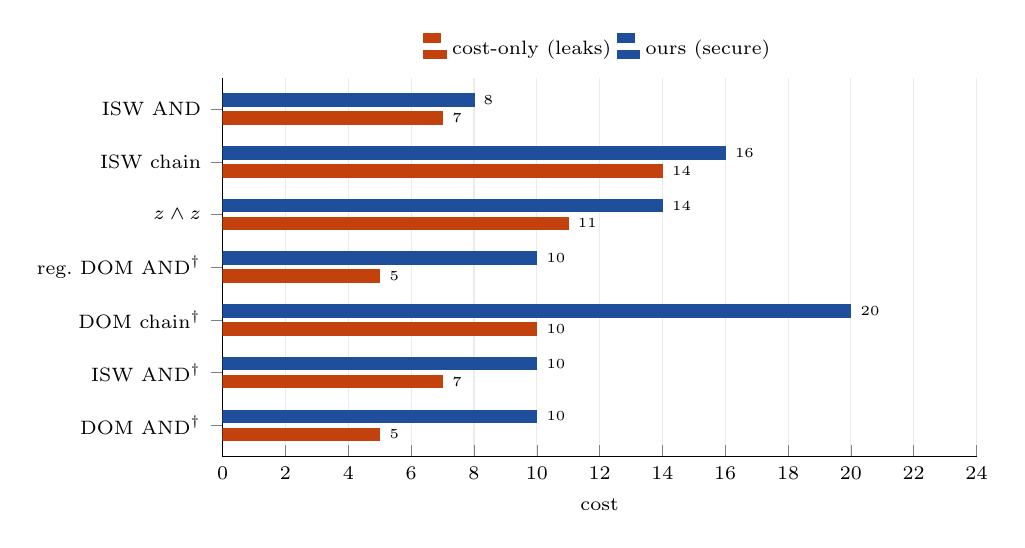
\begin{tikzpicture}
\begin{axis}[xbar,bar width=4.5pt,width=0.92\columnwidth,height=6.4cm,
 xmin=0,xmax=24,xlabel={cost},
 symbolic y coords={domnr,iswnr,domch,domreg,square,chain,isw},ytick=data,
 yticklabels={DOM AND$^\dagger$,ISW AND$^\dagger$,DOM chain$^\dagger$,reg.\ DOM AND$^\dagger$,$z\wedge z$,ISW chain,ISW AND},
 yticklabel style={font=\scriptsize},xticklabel style={font=\scriptsize},label style={font=\scriptsize},
 nodes near coords,nodes near coords style={font=\tiny},
 legend style={font=\scriptsize,at={(0.5,1.02)},anchor=south,draw=none,legend columns=2},
 axis lines*=left,xmajorgrids,grid style={black!8},enlarge y limits=0.1]
\addplot[fill=orange,draw=orange] coordinates {(5,domnr)(7,iswnr)(10,domch)(5,domreg)(11,square)(14,chain)(7,isw)};
\addplot[fill=blue,draw=blue] coordinates {(10,domnr)(10,iswnr)(20,domch)(10,domreg)(14,square)(16,chain)(8,isw)};
\legend{cost-only (leaks),ours (secure)}
\end{axis}
\end{tikzpicture}
\caption{Price of security. Every circuit on which the cost-only optimiser and our tool disagree: the cost-only result always leaks. Costs are gates (ISW AND, chain), gates + random bits ($z\wedge z$), or gates + registers ($^\dagger$, glitch-extended model).}
\label{fig:price}
\end{figure}

\subsection{Cost: ours versus the hand-written design}
Where the starting circuit has waste, the secure result is 20--58\% cheaper: 58\% on \texttt{factor}, 52\% on the multiplexer, 45\% on two ANDs sharing a factor, 40\% on the over-refreshed chain, 37\% on the OR-form majority, 25\% on the HPC1 chain, 21\% on majority and 20\% on the full adder (Fig.~\ref{fig:slack}, Table~\ref{tab:frontend}). On tight designs (the hand-written ISW chain and Keccak $\chi$) it finds nothing to save, and it never returns a circuit that leaks. The PINI route is the one case that costs more, 25--33\% above the ISW-based design, in return for certifying circuits too large to check directly.

\subsection{Head-to-head with AGEMA and COMPRESS}\label{sec:h2h}
We ran both tools on the twelve programs of Tables~\ref{tab:frontend} and~\ref{tab:larger} with two shares, all on one machine (an AMD Ryzen 5 5500U laptop, 12 threads, 5.6\,GB, Linux; Yosys 0.70, GHDL 7.0, COMPRESS commit 26ccd9c, AGEMA commit 3de80c1). COMPRESS was run with its default gadget library at latencies 2 to 4; the multiplier and the OR-form majority have no schedule at latency 2, and every other design it produced passed its own behavioural simulation. Its area is the area of the synthesised design from Yosys with the Nangate45 library, the flow its authors use. AGEMA was run through its Yosys front end with its HPC2 and HPC3 gadgets. Its gadgets are VHDL, which we read with the GHDL plugin of Yosys, so AGEMA's area is measured on the same library, not estimated. All areas are in gate equivalents (GE, 1\,GE $=0.798\,\mu$m$^2$). Table~\ref{tab:h2h} shows the results. As a check, the six programs of the first version of this table give the same COMPRESS gadget counts, random bits and area as before (for example 148.0\,GE on $a\wedge b\oplus a\wedge c$), so our flow reproduces the earlier runs.

\begin{table*}[t]
\caption{Measured Head-to-Head on Twelve Programs (Two Shares, One Machine). Area in GE, Nangate45. ``Gadgets'' Counts Masked AND-Type Gadgets; ``rnd'' Counts Fresh Random Bits}\label{tab:h2h}
\centering\footnotesize
\setlength{\tabcolsep}{4.5pt}
\begin{tabular}{@{}lccccccc@{}}
\toprule
& \multicolumn{2}{c}{seqc (this work)} & \multicolumn{2}{c}{AGEMA} & \multicolumn{3}{c}{COMPRESS}\\
\cmidrule(lr){2-3}\cmidrule(lr){4-5}\cmidrule(l){6-8}
Program & gadgets / rnd & area$^{a}$ & gadgets / rnd$^{b}$ & area$^{c}$ & gadgets / rnd & area & area on seqc's logic$^{d}$\\\midrule
$a\wedge b\oplus a\wedge c$ & 1 / 1 & 12.0 & 1 / 1 & 73.0 & 2 / 2 & 148.0 & \textbf{81.7} ($-$45\%)\\
$z\wedge z$, $z=a\oplus b$ & 1 / 2 & 16.7 & 0 / 0 & 4.0 & 1 / 1 & 70.3 & 70.3 (same)\\
multiplexer & 1 / 1 & 16.0 & 3 / 3 & 207.0 & 2 / 2 & 148.7 & \textbf{108.3} ($-$27\%)\\
full adder & 2 / 2 & 32.0 & 3 / 3 & 237.3 & 2 / 2 & 167.3 & 167.3 (same)\\
majority, 2 AND & 2 / 2 & 22.0 & 4 / 4 & 285.0 & 2 / 2 & 152.0 & 152.0 (same)\\
majority, OR form & 4 / 4 & 59.7 & 4 / 4 & 285.0 & 5 / 9 & 282.3 & 290.7 (+3\%), rnd 9 $\to$ 6\\
2-bit comparator & 4 / 4 & 66.3 & 8 / 8 & 517.7 & 4 / 5 & 275.0 & 279.0 (+1\%)\\
2-bit adder & 4 / 4 & 73.0 & 6 / 6 & 543.7 & 4 / 6 & 302.0 & 302.0 (same)\\
$2{\times}2$ multiplier & 7 / 8 & 58.7 & 6 / 6 & 421.7 & 6 / 10 & 374.7 & 420.0 (+12\%)\\
4:1 multiplexer$^\dagger$ & 3 / 3 & 53.3 & 9 / 9 & 641.3 & 3 / 5 & 213.0 & 213.0 (same)\\
Ascon S-box$^\dagger$ & 5 / 5 & 98.0 & 11 / 11 & 937.0 & 5 / 5 & 440.3 & \textbf{411.7} ($-$6\%)\\
PRESENT S-box & 8 / 8 & 133.7 & 24 / 24 & 1753.7 & 9 / 11 & 627.0 & \textbf{555.7} ($-$11\%)\\
\bottomrule
\multicolumn{8}{@{}p{0.97\textwidth}@{}}{\scriptsize $^{a}$Glitch-free, combinational, no registers and no random-number generator; not directly comparable with the glitch-robust, pipelined designs of AGEMA and COMPRESS. $^{b}$HPC2 (one random bit per gadget). $^{c}$Measured: best of HPC2 and HPC3, AGEMA's VHDL gadgets and pipeline registers synthesised together. $^{d}$COMPRESS run on the Boolean structure seqc chose, each gadget as an AND; COMPRESS keeps its own glitch-robust guarantee, and the first number is its best-latency area. Changes are against the COMPRESS area in the previous column. $^\dagger$seqc with $k=2$.}
\end{tabular}
\end{table*}

Three findings stand out. First, \textbf{seqc needs no more gadgets than either tool on ten of the twelve programs.} It needs strictly fewer than AGEMA on eight and strictly fewer than COMPRESS on four, with ties elsewhere. AGEMA's front end optimises the logic for \emph{unmasked} area, so it turns the multiplexers and the S-boxes into NAND and NOR networks, each gate of which then becomes a masked gadget (24 gadgets for the PRESENT S-box against seqc's 8). COMPRESS keeps the logic exactly as written, so it pays for every AND in the source. The two exceptions are $z\wedge z$, where AGEMA's synthesis applies $x\wedge x=x$ and removes the gadget (a rule we deliberately left out to study the refresh), and the multiplier, where seqc's secure optimum has 7 gadgets and both tools have 6. Second, \textbf{the savings carry over into a glitch-robust flow on some programs, not all}: feeding seqc's chosen logic into COMPRESS makes its design smaller on four programs (by 45\% on $a\wedge b\oplus a\wedge c$, 27\% on the multiplexer, 6\% on the Ascon S-box and 11\% on the PRESENT S-box), the same on five, and larger on three (by 12\% on the multiplier, 3\% on the OR-form majority, where the random bits still drop from 9 to 6, and 1\% on the comparator). Third, seqc's own area is far below the other two, but this is not a fair comparison: it has no registers, no random-number generator and only glitch-free security. Fig.~\ref{fig:h2h} summarises the gadget counts.

\begin{figure}[t]
\centering
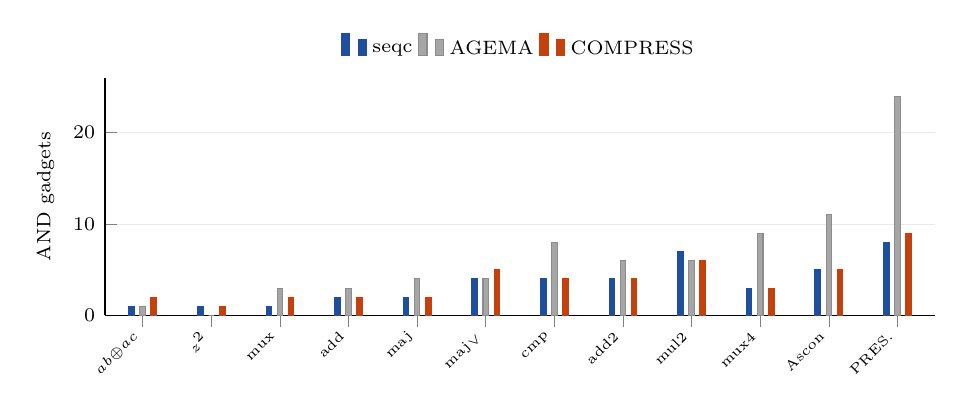
\begin{tikzpicture}
\begin{axis}[ybar,bar width=2pt,width=\columnwidth,height=4.6cm,
 ymin=0,ymax=26,ylabel={AND gadgets},
 symbolic x coords={f,sq,mx,ad,mj,mo,cm,a2,mu,m4,as,pr},xtick=data,
 xticklabels={$ab{\oplus}ac$,$z^2$,mux,add,maj,maj$_\vee$,cmp,add2,mul2,mux4,Ascon,PRES.},
 x tick label style={font=\tiny,rotate=45,anchor=east},yticklabel style={font=\scriptsize},label style={font=\scriptsize},
 legend style={font=\scriptsize,at={(0.5,1.03)},anchor=south,draw=none,legend columns=3},
 axis lines*=left,ymajorgrids,grid style={black!8},enlarge x limits=0.05]
\addplot[fill=blue,draw=blue] coordinates {(f,1)(sq,1)(mx,1)(ad,2)(mj,2)(mo,4)(cm,4)(a2,4)(mu,7)(m4,3)(as,5)(pr,8)};
\addplot[fill=black!35,draw=black!45] coordinates {(f,1)(sq,0)(mx,3)(ad,3)(mj,4)(mo,4)(cm,8)(a2,6)(mu,6)(m4,9)(as,11)(pr,24)};
\addplot[fill=orange,draw=orange] coordinates {(f,2)(sq,1)(mx,2)(ad,2)(mj,2)(mo,5)(cm,4)(a2,4)(mu,6)(m4,3)(as,5)(pr,9)};
\legend{seqc,AGEMA,COMPRESS}
\end{axis}
\end{tikzpicture}
\caption{Masked AND gadgets needed per program (fewer is better). Each gadget costs area and fresh randomness in every masking scheme.}
\label{fig:h2h}
\end{figure}

On speed, all on the machine above, AGEMA takes 8--17\,ms per run and COMPRESS's solver 0.04--0.68\,s over all latencies tried. seqc takes at most 0.2\,s on the five smallest programs and between 6\,s and 132\,s on the larger ones, where its exact checking is the limit (83\,s for the OR-form majority, 75\,s for the 2-bit adder, 132\,s for the PRESENT S-box).

\subsection{Do the savings need equality saturation?}
A fair objection is that any logic minimiser might find the same savings. Table~\ref{tab:noegraph} compares seqc with a plain minimiser, Yosys with ABC mapping to AND and XOR gates, on twelve programs (the six above and the six of Table~\ref{tab:larger}). The minimiser has no idea of masking. It needs more AND gates than seqc on eight programs, the same number on two, and fewer on two: $z\wedge z$, where it applies $x\wedge x=x$, and the multiplier. On eight programs it even needs more ANDs than the source already had, since ABC maps for area, not for the number of ANDs. This is a weak baseline, and a minimiser built to reduce the AND count would do better: for the PRESENT S-box it is known exactly that the minimum number of ANDs is 4 \cite{courtois2011}, against 8 gadgets for seqc and 9 as written. We did not run such a minimiser, and a circuit with the fewest ANDs is not by itself secure, but seqc is clearly not optimal in gadget count there. Table~\ref{tab:noegraph} also gives the area of seqc's own Verilog (Yosys 0.70, Nangate45, 1 GE $=0.798\,\mu$m$^2$, no registers, glitch-free model only). These are the same seqc areas as in Table~\ref{tab:h2h}; they supersede the seqc area column of an earlier version of this table, which came from a different synthesis run.

\begin{table}[t]
\caption{AND Gadgets Without an E-Graph (Yosys/ABC) Versus seqc, and seqc Area}\label{tab:noegraph}
\centering\footnotesize
\setlength{\tabcolsep}{3.2pt}
\begin{tabular}{@{}lrrrrr@{}}
\toprule
Program & Written & ABC & seqc & Rnd. & GE\\\midrule
$a\wedge b\oplus a\wedge c$ & 2 & 1 & 1 & 1 & 12.0\\
$z\wedge z$ & 1 & 0 & 1 & 2 & 16.7\\
multiplexer & 2 & 3 & 1 & 1 & 16.0\\
full adder & 2 & 3 & 2 & 2 & 32.0\\
majority, 2 AND & 2 & 4 & 2 & 2 & 22.0\\
majority, OR form & 5 & 4 & 4 & 4 & 59.7\\
2-bit comparator & 4 & 8 & 4 & 4 & 66.3\\
2-bit adder & 4 & 6 & 4 & 4 & 73.0\\
$2{\times}2$ multiplier & 6 & 6 & 7 & 8 & 58.7\\
4:1 multiplexer$^\dagger$ & 3 & 9 & 3 & 3 & 53.3\\
Ascon S-box$^\dagger$ & 5 & 13 & 5 & 5 & 98.0\\
PRESENT S-box & 9 & 26 & 8 & 8 & 133.7\\
\bottomrule
\multicolumn{6}{@{}p{0.95\columnwidth}@{}}{\scriptsize Written: ANDs in the source (shared terms once). ABC: ANDs after Yosys/ABC. seqc: gadgets and random bits of the secure optimum. $^\dagger$$k=2$.}
\end{tabular}
\end{table}

\subsection{Speed and scale}
Table~\ref{tab:speed} gives the measured run times. Checking each candidate is exact but slows down quickly as circuits grow; PINI extraction and the fast labeller are what make large circuits practical.

\begin{table}[t]
\caption{Measured Speed and Scale}\label{tab:speed}
\centering\footnotesize
\begin{tabularx}{\columnwidth}{@{}>{\raggedright\arraybackslash}Xr@{}}
\toprule
Task & Result\\\midrule
Per-term extraction, ISW chain depth 3 / 4 / 5 & 0.3\,s / 5.4\,s / 133\,s\\
Labeller, depth-5 chain: bit-parallel / reference & 0.4\,s / $\approx$61\,min (est.)\\
PINI extraction, Keccak $\chi$ 32-bit ($2^{128}$ inputs) & 0.05\,s, 545/545 wires\\
PINI extraction, ISW chain depth 15 ($2^{62}$ inputs) & 0.01\,s, 212/212 wires\\
Exact checker, largest input space & $\approx 2^{26}$ points\\
seqc, OR-form majority (5 gadgets), 65 $\to$ 41 & 83\,s\\
Full verification, all 16 steps & $\approx$8\,min (487\,s)\\
\bottomrule
\end{tabularx}
\end{table}

% =====================================================================
\section{Verification}\label{sec:evidence}
% =====================================================================
We never relied on our own checker alone. Every verdict was cross-checked by VerifMSI \cite{meunier2023verifmsi}, a published verifier we did not write, run as a separate program (Table~\ref{tab:oracle}). One command, \code{findings/verify.py -{}-full}, reruns every experiment and checks every number reported here; all 16 steps pass, along with 182 automated tests. Agreement on these circuits is strong evidence, but it is not a proof for every possible circuit. We also tested the verifier itself, and use its exact check, rather than its one-sided symbolic shortcut, as the reference.

\begin{table}[t]
\caption{Agreement With VerifMSI}\label{tab:oracle}
\centering\footnotesize
\begin{tabular}{@{}lrr@{}}
\toprule
Checked & Circuits / wires & Disagree\\\midrule
Exact checker & 1,216 / 21,760 & 0\\
Bit-parallel labeller & 1,265 / 22,463 & 0\\
Value-layer circuits & 27 / 914 & 0\\
Sampled chain extractions & 240 / 6,054 & 0\\
Random PINI-built circuits & 234 / 4,608 & 0\\
Compiled programs & 7 / 178 & 0\\
Larger compiled programs & 6 / 443 & 0\\
Three- and four-share circuits & 6 / 159 & 0\\\midrule
\textbf{Total wire checks} & \textbf{56,579} & \textbf{0}\\\midrule
Glitch checker (probes) & 167 & 0\\
PINI verdicts (gadgets) & 6 & 0\\
\bottomrule
\end{tabular}
\end{table}

% =====================================================================
\section{Related Work}\label{sec:related}
% =====================================================================
\textbf{Masking compilers.} AGEMA \cite{knichel2021agema} turns an unprotected netlist into a masked one using PINI gadgets. It may simplify the \emph{unmasked} logic first, where rewrites cannot hurt security. COMPRESS \cite{cassiers2024compress} and TETRIS \cite{sarma2026tetris} choose and schedule gadgets for a fixed circuit. Tornado \cite{belaid2020tornado} adds refreshes wherever its verifier finds an attack. Feldtkeller et al.\ \cite{feldtkeller2022} let gadgets share random bits, which we do not model. Apart from the search-based work below, none of them explores equivalent \emph{masked} circuits by rewriting. The type-directed compiler of Barthe et al.\ \cite{barthe2016sni} also inserts refreshes automatically, but for a fixed circuit and with a stronger notion (SNI) than the probing notion used here. Kumar et al.\ \cite{kumar2025graph} lower the fresh randomness of first-order masked circuits by graph colouring, and, in their words, only rewire the randomness inputs and leave the logic unchanged.

\textbf{Verifiers.} VerifMSI \cite{meunier2023verifmsi} is our independent referee; maskVerif \cite{barthe2019maskverif} and SILVER \cite{knichel2020silver} are other well-known checkers. superVer \cite{treff2024supver} uses e-graphs to \emph{check} masked circuits rather than optimise them. The authors of the eVer verifier \cite{gourjon2026ever} removed unneeded refreshes from their gadgets by hand; we do this automatically, inside an optimiser.

\textbf{Optimisers that break masking.} MaskedHLS \cite{sarma2024maskedhls} and a study for the German BSI \cite{oberhansl2024study} report that standard synthesis optimisations can recombine shares. MaskedHLS responds by not optimising the logic at all. We explain why this happens in equality saturation, and show how to fix it.

\textbf{E-graphs for hardware.} E-Syn \cite{chen2024esyn} applies equality saturation to gate-level Boolean logic with technology-aware costs and reports area and delay savings over ABC; it has no notion of probing security, so it is the kind of optimiser whose output Finding~1 warns about.

\textbf{Search-based optimisation of masked gadgets.} Koblah et al.\ \cite{koblah2025evo} apply an evolutionary algorithm, with mutation and crossover, to explore alternative gate-level realisations of masked gadgets. Candidates are judged on power and area while functional equivalence and compliance with the probing model are checked, and they report security-preserving reductions of up to 15\% in selected cases. They also report that conventional CAD transformations (technology mapping, FRAIG-based rewriting, retiming) sometimes give large gains but are not systematic under strict masking constraints, which is the situation Finding~1 explains for equality saturation. Their work is the closest to ours in spirit, since it also searches over equivalent masked circuits and keeps secure ones. It differs in what is searched and how: it optimises individual gadgets by randomised search over netlists, whereas we saturate an e-graph (every equivalent form, not a sample), work on whole programs, add a value-level representation for re-sharing, and show which extraction choices are unsafe. We could not confirm from the abstract which verifier or security notion, for example PINI, they use for each candidate; this paper is a preprint (ePrint 2025/1190, latest revision August 2026).

\textbf{What we claim.} We do not claim to be the first to show that optimisers break masking, the first to use e-graphs on masked circuits, the first to search over equivalent masked circuits under a security check, or the first to remove refreshes or choose gadgets. What is new is the analysis and repair inside equality saturation. Since this is a ``nobody has done it'' claim (we searched and found nothing), we rate our confidence as medium.

% =====================================================================
\section{Scope and Limitations}\label{sec:limits}
% =====================================================================
\begin{itemize}
\item \textbf{Scope:} one probe, single-bit circuits without loops; no sharing of random bits between gadgets. The compiler uses two shares; Sec.~\ref{sec:shares} extends only the gadget-level measurement of Finding~1 to $d=3,4$, checked against VerifMSI.
\item \textbf{Savings:} only where the starting circuit has waste; tight designs do not improve.
\item \textbf{Scale:} checking each candidate is exact only among the $k$ cheapest options, and slow on larger circuits; the 0-of-240 result is a sample.
\item \textbf{Glitches:} the PINI result and the generated Verilog assume no glitches.
\item \textbf{Evidence:} no hardware test; the emitted Verilog is synthesised for area and simulated for function on all twelve programs, but no leakage tool was run on it and it assumes no glitches; a head-to-head against AGEMA and COMPRESS on twelve small programs only, one machine, and the proofs are written by hand rather than machine-checked.
\end{itemize}

% =====================================================================
\section{Conclusion}
% =====================================================================
Compiler optimisers promise to keep a program's meaning, and masked hardware needs more than that. Left to minimise cost, equality saturation turns secure masked circuits into cheaper ones that leak, and with two shares this always happens rather than by chance. Checking security when the circuit is chosen fixes this at the wire level. The designers' own tricks need a second, value-level e-graph, where the circuit must be chosen term by term or through PINI to stay safe. The result, seqc, removes waste where there is some and never returns a leaking circuit, and every verdict has been confirmed independently. \textbf{For secure hardware, giving the same answer is not enough: the optimiser must also keep the security.}

\section*{Acknowledgment}
Portions of the code, scripts and this report were prepared with the assistance of an AI system (Claude, Anthropic). The code and data are available at \url{https://github.com/wizard-28/secureeqsat}.

% =====================================================================
\appendices
\section{Proofs}\label{app:proofs}
% =====================================================================
Throughout, a secret $s$ is shared as $(s_0,s_0\oplus s)$ with $s_0$ uniformly random, and all fresh random bits are independent. A wire leaks if what a probe sees on it (its value, or under glitches everything feeding it) has a distribution that depends on the secrets.

\emph{Proof of Proposition~\ref{prop:vplc}.}
(i)~R3 merges $\rf(z)$ into the class of $z$, so $\isw(z,\rf(z))$ and $\isw(z,z)$ become the same node.
(ii)~In $\isw(z,z)$ the wire $z_0\wedge(z_0\oplus z)$ equals $z_0$ when $z=0$ and $0$ when $z=1$, so it leaks.
(iii)~In $\isw(z,\rf(z))$, with $y=(z_0\oplus r',z_1\oplus r')$, each product $z_iy_j$ is the AND of two values that, together, are a reshuffled copy of the uniform pair $(z_0,r')$. It is therefore 1 with probability $1/4$ for either value of $z$. Every other wire is uniform: the input wires because they are shares, and the rest because each contains the gadget's random bit $r$ exactly once.
(iv)~With R3 alone, $z$'s class holds $z$'s own nodes plus the refresh loop. A one-node-per-class extraction cannot follow the loop, so both inputs become the same wire and the result is $\isw(z,z)$.
(v)~Term extraction can follow the loop at one input only, and returns the secure term (cost 14 against 11).\hfill$\square$

\emph{Proof of Proposition~\ref{prop:cut}.}
Let $w$ be a leaking wire in the lowering of a piece $s$ of a larger term $t$. Lowering builds $t$ from its pieces, so the lowering of $t$ contains a wire $w'$ that computes the same function as $w$, up to renaming its random bits, which does not change any distribution. Everything $w'$ depends on lies inside $s$, because the rest of $t$ only uses $s$'s outputs. So a probe on $w'$ sees exactly what a probe on $w$ sees, and $w'$ leaks too. The argument only uses this dependency structure, so it also works when the attacker has several probes. As a sanity check we also enumerated every term over two inputs with up to three operators: all 2,204 leaking terms stay leaking in all 26 one-step contexts each (57,304 checks, no counterexample). This is a bounded check, not a machine-checked proof.\hfill$\square$

\begin{thebibliography}{99}
\footnotesize
\bibitem{willsey2021egg} M.~Willsey, C.~Nandi, Y.~R.~Wang, O.~Flatt, Z.~Tatlock, and P.~Panchekha, ``egg: Fast and extensible equality saturation,'' \emph{Proc. ACM Program. Lang.}, vol.~5, no.~POPL, 2021.
\bibitem{zhang2023egglog} Y.~Zhang, Y.~R.~Wang, O.~Flatt, D.~Cao, P.~Zucker, E.~Rosenthal, Z.~Tatlock, and M.~Willsey, ``Better together: Unifying Datalog and equality saturation,'' \emph{Proc. ACM Program. Lang.}, vol.~7, no.~PLDI, 2023.
\bibitem{ishai2003private} Y.~Ishai, A.~Sahai, and D.~Wagner, ``Private circuits: Securing hardware against probing attacks,'' in \emph{CRYPTO 2003}, LNCS vol.~2729, pp.~463--481, 2003.
\bibitem{gross2016dom} H.~Gro\ss, S.~Mangard, and T.~Korak, ``Domain-oriented masking: Compact masked hardware implementations with arbitrary protection order,'' IACR Cryptol. ePrint Arch., Rep.~2016/486, 2016.
\bibitem{cassiers2020hpc} G.~Cassiers, B.~Gr\'egoire, I.~Levi, and F.-X.~Standaert, ``Hardware private circuits: From trivial composition to full verification,'' \emph{IEEE Trans. Comput.}, 2020.
\bibitem{faust2018robust} S.~Faust, V.~Grosso, S.~Merino Del Pozo, C.~Paglialonga, and F.-X.~Standaert, ``Composable masking schemes in the presence of physical defaults and the robust probing model,'' \emph{IACR TCHES}, vol.~2018, no.~3, pp.~89--120, 2018.
\bibitem{mangard2005glitch} S.~Mangard, T.~Popp, and B.~M.~Gammel, ``Side-channel leakage of masked CMOS gates,'' in \emph{CT-RSA 2005}, LNCS vol.~3376, pp.~351--365, 2005.
\bibitem{cassiers2020pini} G.~Cassiers and F.-X.~Standaert, ``Trivially and efficiently composing masked gadgets with probe isolating non-interference,'' \emph{IEEE Trans. Inf. Forensics Secur.}, vol.~15, pp.~2542--2555, 2020.
\bibitem{suciu2025semantic} D.~Suciu, Y.~R.~Wang, and Y.~Zhang, ``Semantic foundations of equality saturation,'' in \emph{ICDT 2025}, LIPIcs vol.~328, 2025.
\bibitem{belaid2020tornado} S.~Bela\"id, P.-\'E.~Dagand, D.~Mercadier, M.~Rivain, and R.~Wintersdorff, ``Tornado: Automatic generation of probing-secure masked bitsliced implementations,'' in \emph{EUROCRYPT 2020}, 2020.
\bibitem{knichel2021agema} D.~Knichel, A.~Moradi, N.~M\"uller, and P.~Sasdrich, ``Automated generation of masked hardware,'' \emph{IACR TCHES}, vol.~2022, no.~1, pp.~589--629, 2022.
\bibitem{meunier2023verifmsi} Q.~L.~Meunier and A.~Taleb, ``VerifMSI: Practical verification of hardware and software masking schemes implementations,'' in \emph{SECRYPT 2023}, pp.~520--527, 2023.
\bibitem{gourjon2026ever} M.~Gourjon, M.~Orlt, P.~Pauls, and A.~Treff, ``eVer: Universal and automated verification of side-channel security for additive, inner product, polynomial and general code-based masking,'' IACR Cryptol. ePrint Arch., Rep.~2026/208, 2026.
\bibitem{sarma2024maskedhls} N.~Sarma, A.~S.~Thakur, and C.~Karfa, ``MaskedHLS: Domain-specific high-level synthesis of masked cryptographic designs,'' \emph{IEEE TCAD}, vol.~43, no.~11, pp.~3973--3984, 2024.
\bibitem{treff2024supver} A.~Treff, P.~Pauls, M.~Orlt, and M.~Gourjon, ``superVer: Verifying probabilistic independence of systems of expressions using equality saturation,'' work-in-progress abstract, \emph{EGRAPHS 2024}, 2024.
\bibitem{feldtkeller2022} J.~Feldtkeller, D.~Knichel, P.~Sasdrich, A.~Moradi, and T.~G\"uneysu, ``Randomness optimization for gadget compositions in higher-order masking,'' \emph{IACR TCHES}, vol.~2022, no.~4, pp.~188--227, 2022.
\bibitem{cassiers2024compress} G.~Cassiers, B.~Gigerl, S.~Mangard, C.~Momin, and R.~Nagpal, ``Compress: Generate small and fast masked pipelined circuits,'' \emph{IACR TCHES}, vol.~2024, no.~3, pp.~500--529, 2024.
\bibitem{sarma2026tetris} N.~Sarma, T.~Patidar, N.~Brahamanya, and C.~Karfa, ``TETRIS: Automated design space exploration of randomness--latency trade-offs in masked hardware,'' IACR Cryptol. ePrint Arch., Rep.~2026/1306, 2026.
\bibitem{barthe2019maskverif} G.~Barthe \emph{et al.}, ``MaskVerif: Automated verification of higher-order masking in presence of physical defaults,'' in \emph{ESORICS 2019}, pp.~300--318, 2019. % UNVERIFIED: full author list (HAL page blocked, search snippets disagree); fetch before submission.
\bibitem{barthe2016sni} G.~Barthe, S.~Bela\"id, F.~Dupressoir, P.-A.~Fouque, B.~Gr\'egoire, P.-Y.~Strub, and R.~Zucchini, ``Strong non-interference and type-directed higher-order masking,'' in \emph{ACM CCS 2016}, pp.~116--129, 2016.
\bibitem{knichel2020silver} D.~Knichel, P.~Sasdrich, and A.~Moradi, ``SILVER -- Statistical independence and leakage verification,'' in \emph{ASIACRYPT 2020}, LNCS, pp.~787--816, 2020.
\bibitem{chen2024esyn} C.~Chen, G.~Hu, D.~Zuo, C.~Yu, Y.~Ma, and H.~Zhang, ``E-Syn: E-graph rewriting with technology-aware cost functions for logic synthesis,'' in \emph{Proc. DAC}, 2024, arXiv:2403.14242.
\bibitem{kumar2025graph} Dilip Kumar S.~V., B.~Gierlichs, and I.~Verbauwhede, ``A graph-theoretic framework for randomness optimization in first-order masked circuits,'' IACR Cryptol. ePrint Arch., Rep.~2025/2102, 2025.
\bibitem{koblah2025evo} D.~S.~Koblah, D.~M.~Mehta, N.~Poch, M.~Hashemi, F.~Ganji, and D.~Forte, ``Towards AI-driven optimization of robust probing model-compliant masked hardware gadgets using evolutionary algorithms,'' IACR Cryptol. ePrint Arch., Rep.~2025/1190, 2025 (revised Aug. 2026), preprint.
\bibitem{courtois2011} N.~T.~Courtois, D.~Hulme, and T.~Mourouzis, ``Solving circuit optimisation problems in cryptography and cryptanalysis,'' preprint hosted by the IMA, 2011. % UNVERIFIED: venue; the claim used (multiplicative complexity of the PRESENT S-box is exactly 4, Theorem 1) was read in the document.
\bibitem{oberhansl2024study} F.~Oberhansl, T.~Stelzer, and M.~Schink, ``New study on the synthesis of cryptographic hardware implementations,'' Fraunhofer AISEC, commissioned by the BSI, Nov. 2024.
\end{thebibliography}

\end{document}
